
The core formalistm and all the necessary steps towards building a PDF to describe the amplitude properties and anguular structure of \BJpsiKst decays are presented in
the current section. A brief discription of the angular pdf derivation is given in \secref{Diferential_Decay_Rate}.
Treatment of the angular acceptance are addressed in \secref{Accceptance} and \secref{Accceptance_Corrections}.
In \secref{Kpi_Invariant_mass} the implications arising from the \mkpi dependance are discussed.
The effect of assymetries introduced by detector imperfections such as productiuon and detection assymetries are delat with
in \secref{experimentalAssym}. Some aspects of the maximum likelihood fit are presented in \secref{Simutaneous_Likelihood_ fit},
along with the \ACP parameters of interest, which are introduced in a special way in angular fit when building the full decay rate \pdf.


%%%%%%%%%%%%%%%%%%%%%%%%%%%%%%%%%%%%%%
\subsection{Angular Dependence}
\label{Diferential_Decay_Rate}
%%%%%%%%%%%%%%%%%%%%%%%%%%%%%%%%%%%%%%
The decay of intreast, \BJpsiKst, is a P2VV process\footnote{P2VV is an acronim that characterises the spin-parity of the particles involved in the dacay.
The $\Bs$ (and $\Bd$) is spin-0 parity minus (Pseudoscalar) particle, whereas the intermediate resonances $\Jpsi$ and $\phi$ are spin-1 parity minus (Vector) particles. Hence the
acronim P2VV.} with 4 particles in the final state. There are at least two ways to describe the angular dependence of that decay, namelly the transversity framework \cite{transvFrameworkI,transvFrameworkII}
and the helicity formalism \cite{helicityFormI,helicityFormII}. In both cases the goal is to come up with an angular dependant description of the total decay amplitude.
In the transversity framework the decay amplitude is decomposed to the three possible polarization states of the intermediate particles \Jpsi and \Kst with respect to 
the \Bs rest frame using polarization vetors of the decay amplitude. For the current analysis the helicity formalism is addopted where the angular dependance is 
introduced by summing all possible spin conficurations of the intermediate vector paticles relative to their momentum direction in the \Bs rest mass frame
and squaring the sum. Or in more comapct wording, from summing up all possible helicity configurations of the intermediate vecror particles. A detailed derivation of both 
approaches within the scope of a P2VV decay can be found in \cite{daanThesis} and \cite{jeroenThesis} respectivelly for the trasvercity and helicity formalism.

\begin{table}[!h]
  \centering 
  \caption{ Angular functions corresponding to each term in \equref{ang_terms} for the \BJpsiKst decay. Pure and interference \pwave terms are shown in the upper part, 
    whereas the \swave plus \spwave interference in the lower. The angular functions are expressed in the helicity basis. The angles $\cos\thetaK,\cos\thetamu,\phihel$
    are called \emph{helicity angles} and in \figref{helAngles} are put into perspective. The $P$ and $Y$ symbols denote ascosiated legendre polynomials and real valued sperical harmonics
    respectively. The middle column express the angular dependence in an orthogonal basis and it is equivalent to the last column. }
  \renewcommand{\arraystretch}{1.2}
  \label{ang_distr}
  \begin{tabular}{ccc}
    \hline
    $a_n$                             &
    %$hh'$                                  &
      $h_n(\Omega) \times 16\sqrt{\pi}$      &
      $h_n(\Omega) \times \tfrac{32\pi}{9}$  \\

    \hline
    $\AmpSq{0}$  &
    %00  &
      $4\, (P_0^0 + 2\, P_2^0)\, (Y_{0,\,0} - \tfrac{1}{\sqrt{5}}\, Y_{2,\,0})$  &
      $2\, \cos^2\thetaK\, \sin^2\thetamu$  \\

    $\AmpSq{\parallel}$  &
    %$\parallel\parallel$  &
      $P_2^2\, (2\, Y_{0,\,0} + \tfrac{1}{\sqrt{5}}\, Y_{2,\,0} - \sqrt{\tfrac{3}{5}}\, Y_{2,\,+2})$  &
      $\sin^2\thetaK\, (1 - \sin^2\thetamu\, \cos^2\phihel)$  \\

    $\AmpSq{\perp}$  &
    %$\perp\perp$  &
      $P_2^2\, (2\, Y_{0,\,0} + \tfrac{1}{\sqrt{5}}\, Y_{2,\,0} + \sqrt{\tfrac{3}{5}}\, Y_{2,\,+2})$  &
      $\sin^2\thetaK\, (1 - \sin^2\thetamu\, \sin^2\phihel)$  \\

    $\ReAmp{0}{\parallel}$  &
    %0$\parallel$ ($\Re$)  &
      $+2\sqrt{2}\sqrt{\tfrac{3}{5}}\, P_2^1\, Y_{2,\,+1}$  &
      $+\frac{1}{\sqrt{2}}\, \sin2\thetaK\, \sin2\thetamu\, \cos\phihel$  \\

    $\ImAmp{0}{\perp}$  &
    %0$\perp$ ($\Im$)  &
      $-2\sqrt{2}\sqrt{\tfrac{3}{5}}\, P_2^1\, Y_{2,\,-1}$  &
      $-\frac{1}{\sqrt{2}}\, \sin2\thetaK\, \sin2\thetamu\, \sin\phihel$  \\


    $\ImAmp{\parallel}{\perp}$  &
    %$\parallel\perp$ ($\Im$)  &
      $+2\sqrt{\tfrac{3}{5}}\, P_2^2\, Y_{2,\,-2}$  &
      $+\sin^2\thetaK\, \sin^2\thetamu\, \sin2\phihel$  \\

    \hline
    $\AmpSq{{\text{S}}}$  &
      $4\, P_0^0\, (Y_{0,\,0} - \tfrac{1}{\sqrt{5}}\, Y_{2,\,0})$  &
      $\tfrac{2}{3}\, \sin^2\thetamu$  \\

    $\ReAmp{0}{{\text{S}}}$  &
      $8\sqrt{3}\, P_1^0\, (Y_{0,\,0} - \tfrac{1}{\sqrt{5}}\, Y_{2,\,0})$  &
      $\tfrac{4}{3}\sqrt{3}\, \cos\thetaK\, \sin^2\thetamu$  \\

    $\ReAmp{\parallel}{{\text{S}}}$  &
      $+6\sqrt{2}\tfrac{1}{\sqrt{5}}\, P_1^1\, Y_{2,\,+1}$  &
      $+\tfrac{1}{3}\sqrt{6}\, \sin\thetaK\, \sin2\thetamu\, \cos\phihel$  \\

    $\ImAmp{\perp}{{\text{S}}}$  &
      $+6\sqrt{2}\tfrac{1}{\sqrt{5}}\, P_1^1\, Y_{2,\,-1}$  &
      $+\tfrac{1}{3}\sqrt{6}\, \sin\thetaK\, \sin2\thetamu\, \sin\phihel$  \\
    \hline
  \end{tabular}
\end{table}  
 
The current paragraph aims at very briefly explaining the steps needed to arive to an expression for the angular decay rate for \BsJpsiKst decays, which is the sum of ten terms.  

\begin{align}
  \frac{d\Gamma(\text{\BJpsiKst})}{d\Omega\;d\mkpi} \propto |\mathcal{A}&(\text{\BJpsiKst})|^2 = \nonumber \\
                                                    &= \left| \sum_i^{0,\parallel,\perp,S} A_i(\Omega,\mkpi) \right|^2  \propto \sum_n a_n h_n \mKpiAmp
  \label{ang_terms}
\end{align}

\noindent Where the term $\mathcal{A}(\text{\BJpsiKst})$ is the amplitude of the decay which is decomposited in its \pwave ($0$, $\parallel$, $\perp$) and \swave ($S$) polarizations.
The terms $a_n$ come from squaring the amplitude and their exact espresions are shown in the first column of 
\tabref{ang_distr}\footnote{It is intreasting to see in \cite{jeroenThesis} how the $\Re$ and $\Im$ parts of the itnerference terms show up.}. 
Note the appearence of \pwave self interference and \spwave interference terms. The functions $h$ represent the angular dependance of each term, whereas $\mKpiAmp$ stands 
for the \mkpi dependence of the anplitude and its special treatment is postponed for the next section. \tabref{ang_distr} lists the angular part of the decay rate 
(meaning the $h$ functions) equation which is the result of appling the \emph{helicity formalistm} in the \BJpsiKst decay. The compact
notation $\Omega$ stands for the so called \emph{heliciy angles}. Three angles are required in a 4 body decay which along with the \mkpi
total the degrees of freadom neccessaty to describe such a system. Those angles are $\thetaK,\thetamu,\phihel$ and are defined in \figref{helAngles}. 
In that figure it can be seen that $\thetamu$ is the angle of the positive $\mu$ with respect to the momentum of the \Jpsi in the \Bs rest frame.
Similarly for $\thetaK$, the \kaon is used to define the angle with respect to the momentum of the intermediate \Kpi resonance. Finally $\phihel$ is 
the relative angle between the \Kpi and dimuon decay plances, where each plane is again defined in the rest frame of the respective intermediate resonance.  

Lastly, the mathematically elegant orthogonal angular basis of $P$ and $Y$
\footnote{The decompotition of angular functions in an orthogonal basis follows naturally from the fact that sperical harmonics can be expressed as 
Wigner-$D$ matrices. More details on this mapping can be found in \cite{jeroenThesis} } 
is adopted in the current analysis, since the integrals of type $\int_{-1}^{1}Pd\cos\thetaK$ and $\int_{\cos\theta=-1,\varphi=-\pi}^{\cos\theta=1,\varphi=\pi}Yd\cos\theta d\varphi$ are known 
analitically thus significantly reducing the fiting time and simplifing the implementation of the angular fucntions.


\begin{figure}[h]
\begin{center}
  \includegraphics[width=\textwidth]{Figures/Chapter4/helAngles.pdf}
  \caption{Definition of the decay angles in the helicity formalism.}
  \label{helAngles}  
\end{center}
\end{figure}


%%%%%%%%%%%%%%%%%%%%%%%%%%%%%%%%%%%%%%
\subsection{Acceptance}
\label{Accceptance}
%%%%%%%%%%%%%%%%%%%%%%%%%%%%%%%%%%%%%%
While the effects of angular resolution are known to be negligible for this analysis, angular acceptance on the other hand can
not be neglected. The current section introduces the acceptance shape. After that the parametriation of the acceptance is discussed
and finally an important issue relaeted to the choice of parametrizations is dealt with.

The shape of the acceptance can be seen in \figref{angAcc_ctk} to \figref{angAcc_phi}. The most striging feature is the drop of efficiency 
close to $\cos\thetaK=1$, which implies that the pion is more likely to fly out of the geometrical acceptance of the detector
and thus not be reconstruted compared to a kaon. This feature can be understood given the  definition of $\cos\thetaK$ in \figref{helAngles}. 
The scenario where $\cos\thetaK\rightarrow 1$ and hence $\thetaK \rightarrow 0$ correponds to a soft pion after boosting
to the lab frame. Since the pion is lighter that a kaon it is more likely that it flyies out of the acceptace more
often than a kaon does, creating the observed assymetric efficiency loss in the $\cos\thetaK$ projection. With that said, it is intuitive that
this type of efficiency loss is driven by the mass diffference between the two particles. In the case of the $\cos\thetamu$ the
reconstruction iduced inefficiency described before is symmetric with respect to the positive and negative muons since they have the same mass.
As for acceptance in $\phihel$ it is very close to being flat. By staring again \figref{helAngles} one does not expect any
reason for a strong acceptance effect in that projection. In addition to this type of acceptance effects any of the selection 
cuts applied could also introduce some ineeficiency.  

\begin{figure}[h]
  \centering
  \begin{subfigure}{0.49\textwidth}
    \tikzsetnextfilename{helcosthetaK_allKaons_binall}
    \scalebox{1.3}{\input{Figures/Chapter4/helcosthetaK_allKaons_binall}}
    \caption{}
    \label{angAcc_ctk}
  \end{subfigure}%
  \hfill%
  \begin{subfigure}{0.49\textwidth}
    \tikzsetnextfilename{helcosthetaL_allKaons_binall}
    \scalebox{1.3}{\input{Figures/Chapter4/helcosthetaL_allKaons_binall}}
    \caption{}
    \label{angAcc_ctl}
  \end{subfigure}

  \vspace*{0.02\textwidth}
  \begin{subfigure}{0.49\textwidth}
    \tikzsetnextfilename{helphi_allKaons_binall}
    \scalebox{1.3}{\input{Figures/Chapter4/helphi_allKaons_binall}}
    \caption{}
    \label{angAcc_phi}
  \end{subfigure}
  \caption{Angular acceptance shape from simulated data. Each event in the simulated sample has been weighted with the inverse integral 
           of the \pdf that was used to generate them, resulting tothose three distributions that give a feeling of the acceptance shape.
           The scale of the $y$-axis is arbitrary.}
\end{figure}

\subsubsection{Acceptance parametrization}
As for the parametrization of the angular acceptance there are at least two ways to proceed.
namelly the \emph{efficiency moments} \cite{jeroenThesis} and the \emph{normalization weights} \cite{tristanThesis,jeroenThesis}. 
The current analysis implements the first one, where the efficiency function is parametrised using orthogonal functions (nicely
combined with the angular description formalism in the previous subsection). Such a parameterization can be seen in the next equation 
\equref{eff_func}. The symbol $\effbase$ is introduced as a shorter notation.

\begin{center}
\begin{equation}
  \epsilon(\Omega) = \sum_{ijk} \; \moment{i}{j}{k} \; P_i^0(\cos\thetaK) \; Y_{jk}(\cos\thetamu,\phihel) \equiv \moment{i}{j}{k} \; \effbase
  \label{eff_func}
\end{equation}
\end{center}

\noindent where the familiar from the previous section spherical harmonics ($Y$) and ascosiated legender polynimials ($P$) show up as the basis
functions on which the angular acceptance is decomposed to by means of the basis coeeficients $c^i_{k}$, hearafter efficicney moments (or simply moments). 
The reason of choosing the particular parametrizations is obisously for the known anlytical integals of product of two $P$ or $Y$. 
Following the above parametrizations one just needs to choose a set of $c^i_{jk}$ and find a way compute them. In principle there are infinite efficiency moments
since the sum in \equref{eff_func} runs through all possible values of the $ijk$ indices. However in practice only a small number of efficiency moments 
contribute significantly to the propper description of the angular acceptance shape. The efficiency moments used to describe the acceptance 
shape are shown in the first column of \tabref{eff_moms_table}. The choice of those particular moments is connected to an important issue with the acceptance 
structure close to $\cos\thetaK=1$ and it is addressed at the end of the current section.   

In order for the efficiency moments $c^i_{jk}$ to be computed a definition of the efficiency is necesary. Note that this computation relies on 
simulated data where all the generating conditions are known. The efficiency then is defined as the ratio of two angular dependant \pdfs, namelly
\Pobs and \Pgen. The first is the angular \pdf that the simulated data follow after all stages of reconstruction and offline selection, whereas
the later is the angular \pdf which the Monte Carlo data have been generated with. It follows that the efficiency is defined as the ratio of the first
over the later and it is shown in equation \equref{eff_def}.

\begin{center}
\begin{equation}
  \epsilon(\Omega) \equiv \frac{\Pobs}{\Pgen}
  \label{eff_def}
\end{equation}
\end{center}

\noindent Computing the efficiency moments is done by projecting the efficiency as defined in \equref{eff_def} on the orthogonal $P\;Y$ basis.
This projection is shown in \equref{eff_moms_def}. Where the factor $j+\frac{1}{2}$ is used to acount for the fact that the ascosiated legender 
polynomials form an orthogonal basis but in fact the orthonormal behaviour is rquired to properly compute the efficiency moments. 


\begin{center}
\begin{align}
   c^i_{jk}  \equiv &(j + \frac{1}{2}) \; \int \; d\Omega \; \effbase \; \epsilon(\Omega) \nonumber \\ 
                 = &(j + \frac{1}{2}) \; \int \; d\Omega \; \effbase \; \frac{\Pobs}{\Pgen}
  \label{eff_moms_def}
\end{align}
\end{center}

\noindent The last step in the calculation of the efficiency moments is the computation of the integral in \equref{eff_moms_def}.
This is done by means of simulated data and the integral is computed following the concept of Monte Carlo integration. This implies
that the integral in \equref{eff_moms_def} can be estimated by a sum over the simulated data (which they have passed through the same 
steps of reconstruction and offline selection as the real data) as shown in \equref{eff_moms_calc}.   

\begin{center}
\begin{equation}
  E\left[ \int \; d\Omega \; \effbase \frac{\Pobs}{\Pgen} \right] = \frac{1}{\Nobs} \sum_e^{\Nobs} \frac{\effbase}{\Pgen}  
  \label{eff_moms_calc}
\end{equation}
\end{center}

\noindent Combining \equref{eff_moms_def} and \equref{eff_moms_calc} the final expresion for computing the efficiency moments is shown
in \equref{eff_moms_calc_final} and the result of the computations can be found it table \tabref{eff_moms_calc_final}  

\begin{center}
\begin{equation}
 c^i_{jk} \equiv (j + \frac{1}{2})  \frac{1}{\Nobs} \sum_e^{\Nobs} \frac{\effbase}{\Pgen}  
  \label{eff_moms_calc_final}
\end{equation}
\end{center}

\begin{table}[h]
  \centering 
  \caption{ Efficiency moments. }
  \renewcommand{\arraystretch}{1.2}
  \label{eff_moms_table}
  \begin{tabular}{ccc}
    \hline
    moment & central value & standard deviation \\
    \hline
    $\moment{0}{0}{0}$ & +3.7785  & 0.0016 \\
    $\moment{1}{0}{0}$ & -2.1268  & 0.0059 \\
    $\moment{2}{0}{0}$ & -1.9557  & 0.0089 \\
    $\moment{3}{0}{0}$ & +0.0009  & 0.0106 \\    
    $\moment{4}{0}{0}$ & +0.1461  & 0.0122 \\
    $\moment{5}{0}{0}$ & +0.1095  & 0.0134 \\
    
    $\moment{0}{2}{0}$ & +0.2822  & 0.0046 \\
    $\moment{0}{2}{2}$ & +0.0505  & 0.0040 \\
    $\moment{0}{4}{0}$ & +0.0838  & 0.0046 \\

    $\moment{1}{4}{0}$ & -0.0603  & 0.0081 \\
    $\moment{2}{2}{0}$ & -0.1139  & 0.0111 \\
    $\moment{2}{2}{2}$ & -0.0453  & 0.0082 \\
\hline
  \end{tabular}
\end{table}  


\subsubsection{Choice of efficiency moments}
The choice of efficiency moments has to do with the structure of the acceptance at $\cos\thetaK=1$. At that point the acceptance goes to zero
which is not a problem by itself. However within the parametrization that is adopted in this analysis it can happen that the acceptance fucntion
\equref{eff_func} can take negative values depending on the choice of ceratain efficiency moments. In other words the approach of efficiency moments does
not guarantee that the acceptance shape discribed by the same equation is a positive definite quantity. Note that this is an artifact of the parametrization
and by no means is there something wrong in the data or the detector. The problem is mathematical in nature and there is no standard solution known
to the author when those lines are being written. The approach followed to solve this problem has two steps. First a constrain on the acceptance function, \equref{eff_func}, is 
introduced to force its value positive and second a constrained fit to the efficiency moments is performed to optimise the acceptance shape discription.
The result is a hybrid acceptance function that is positive definite.

\begin{figure}[h]
  \centering
  \begin{subfigure}{0.5\textwidth}
    \tikzsetnextfilename{eff_helcosthetaK_neg_all_raw_zoom}
    \scalebox{1.3}{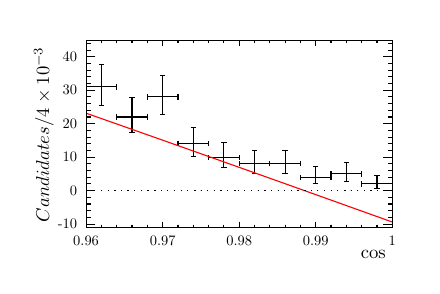
\begin{tikzpicture}
\pgfdeclareplotmark{cross} {
\pgfpathmoveto{\pgfpoint{-0.3\pgfplotmarksize}{\pgfplotmarksize}}
\pgfpathlineto{\pgfpoint{+0.3\pgfplotmarksize}{\pgfplotmarksize}}
\pgfpathlineto{\pgfpoint{+0.3\pgfplotmarksize}{0.3\pgfplotmarksize}}
\pgfpathlineto{\pgfpoint{+1\pgfplotmarksize}{0.3\pgfplotmarksize}}
\pgfpathlineto{\pgfpoint{+1\pgfplotmarksize}{-0.3\pgfplotmarksize}}
\pgfpathlineto{\pgfpoint{+0.3\pgfplotmarksize}{-0.3\pgfplotmarksize}}
\pgfpathlineto{\pgfpoint{+0.3\pgfplotmarksize}{-1.\pgfplotmarksize}}
\pgfpathlineto{\pgfpoint{-0.3\pgfplotmarksize}{-1.\pgfplotmarksize}}
\pgfpathlineto{\pgfpoint{-0.3\pgfplotmarksize}{-0.3\pgfplotmarksize}}
\pgfpathlineto{\pgfpoint{-1.\pgfplotmarksize}{-0.3\pgfplotmarksize}}
\pgfpathlineto{\pgfpoint{-1.\pgfplotmarksize}{0.3\pgfplotmarksize}}
\pgfpathlineto{\pgfpoint{-0.3\pgfplotmarksize}{0.3\pgfplotmarksize}}
\pgfpathclose
\pgfusepathqstroke
}
\pgfdeclareplotmark{cross*} {
\pgfpathmoveto{\pgfpoint{-0.3\pgfplotmarksize}{\pgfplotmarksize}}
\pgfpathlineto{\pgfpoint{+0.3\pgfplotmarksize}{\pgfplotmarksize}}
\pgfpathlineto{\pgfpoint{+0.3\pgfplotmarksize}{0.3\pgfplotmarksize}}
\pgfpathlineto{\pgfpoint{+1\pgfplotmarksize}{0.3\pgfplotmarksize}}
\pgfpathlineto{\pgfpoint{+1\pgfplotmarksize}{-0.3\pgfplotmarksize}}
\pgfpathlineto{\pgfpoint{+0.3\pgfplotmarksize}{-0.3\pgfplotmarksize}}
\pgfpathlineto{\pgfpoint{+0.3\pgfplotmarksize}{-1.\pgfplotmarksize}}
\pgfpathlineto{\pgfpoint{-0.3\pgfplotmarksize}{-1.\pgfplotmarksize}}
\pgfpathlineto{\pgfpoint{-0.3\pgfplotmarksize}{-0.3\pgfplotmarksize}}
\pgfpathlineto{\pgfpoint{-1.\pgfplotmarksize}{-0.3\pgfplotmarksize}}
\pgfpathlineto{\pgfpoint{-1.\pgfplotmarksize}{0.3\pgfplotmarksize}}
\pgfpathlineto{\pgfpoint{-0.3\pgfplotmarksize}{0.3\pgfplotmarksize}}
\pgfpathclose
\pgfusepathqfillstroke
}
\pgfdeclareplotmark{newstar} {
\pgfpathmoveto{\pgfqpoint{0pt}{\pgfplotmarksize}}
\pgfpathlineto{\pgfqpointpolar{44}{0.5\pgfplotmarksize}}
\pgfpathlineto{\pgfqpointpolar{18}{\pgfplotmarksize}}
\pgfpathlineto{\pgfqpointpolar{-20}{0.5\pgfplotmarksize}}
\pgfpathlineto{\pgfqpointpolar{-54}{\pgfplotmarksize}}
\pgfpathlineto{\pgfqpointpolar{-90}{0.5\pgfplotmarksize}}
\pgfpathlineto{\pgfqpointpolar{234}{\pgfplotmarksize}}
\pgfpathlineto{\pgfqpointpolar{198}{0.5\pgfplotmarksize}}
\pgfpathlineto{\pgfqpointpolar{162}{\pgfplotmarksize}}
\pgfpathlineto{\pgfqpointpolar{134}{0.5\pgfplotmarksize}}
\pgfpathclose
\pgfusepathqstroke
}
\pgfdeclareplotmark{newstar*} {
\pgfpathmoveto{\pgfqpoint{0pt}{\pgfplotmarksize}}
\pgfpathlineto{\pgfqpointpolar{44}{0.5\pgfplotmarksize}}
\pgfpathlineto{\pgfqpointpolar{18}{\pgfplotmarksize}}
\pgfpathlineto{\pgfqpointpolar{-20}{0.5\pgfplotmarksize}}
\pgfpathlineto{\pgfqpointpolar{-54}{\pgfplotmarksize}}
\pgfpathlineto{\pgfqpointpolar{-90}{0.5\pgfplotmarksize}}
\pgfpathlineto{\pgfqpointpolar{234}{\pgfplotmarksize}}
\pgfpathlineto{\pgfqpointpolar{198}{0.5\pgfplotmarksize}}
\pgfpathlineto{\pgfqpointpolar{162}{\pgfplotmarksize}}
\pgfpathlineto{\pgfqpointpolar{134}{0.5\pgfplotmarksize}}
\pgfpathclose
\pgfusepathqfillstroke
}
\definecolor{c}{rgb}{1,1,1};
\draw [color=c, fill=c] (0.1,3.20034) rectangle (4.9,6.21242);
\draw [color=c, fill=c] (0.772,3.68227) rectangle (4.66,6.06181);
\definecolor{c}{rgb}{0,0,0};
\draw [c] (0.772,3.68227) -- (0.772,6.06181) -- (4.66,6.06181) -- (4.66,3.68227) -- (0.772,3.68227);
\draw [c,line width=0.4] (0.772,3.68227) -- (4.66,3.68227);
\draw [anchor= east] (4.66,3.34492) node[scale=0.672711, rotate=0]{$\cos\thetaK$};
\draw [c,line width=0.4] (0.772,3.75546) -- (0.772,3.68227);
\draw [c,line width=0.4] (0.9664,3.71887) -- (0.9664,3.68227);
\draw [c,line width=0.4] (1.1608,3.71887) -- (1.1608,3.68227);
\draw [c,line width=0.4] (1.3552,3.71887) -- (1.3552,3.68227);
\draw [c,line width=0.4] (1.5496,3.71887) -- (1.5496,3.68227);
\draw [c,line width=0.4] (1.744,3.75546) -- (1.744,3.68227);
\draw [c,line width=0.4] (1.9384,3.71887) -- (1.9384,3.68227);
\draw [c,line width=0.4] (2.1328,3.71887) -- (2.1328,3.68227);
\draw [c,line width=0.4] (2.3272,3.71887) -- (2.3272,3.68227);
\draw [c,line width=0.4] (2.5216,3.71887) -- (2.5216,3.68227);
\draw [c,line width=0.4] (2.716,3.75546) -- (2.716,3.68227);
\draw [c,line width=0.4] (2.9104,3.71887) -- (2.9104,3.68227);
\draw [c,line width=0.4] (3.1048,3.71887) -- (3.1048,3.68227);
\draw [c,line width=0.4] (3.2992,3.71887) -- (3.2992,3.68227);
\draw [c,line width=0.4] (3.4936,3.71887) -- (3.4936,3.68227);
\draw [c,line width=0.4] (3.688,3.75546) -- (3.688,3.68227);
\draw [c,line width=0.4] (3.8824,3.71887) -- (3.8824,3.68227);
\draw [c,line width=0.4] (4.0768,3.71887) -- (4.0768,3.68227);
\draw [c,line width=0.4] (4.2712,3.71887) -- (4.2712,3.68227);
\draw [c,line width=0.4] (4.4656,3.71887) -- (4.4656,3.68227);
\draw [c,line width=0.4] (4.66,3.75546) -- (4.66,3.68227);
\draw [anchor=base] (0.772,3.45937) node[scale=0.52322, rotate=0]{0.96};
\draw [anchor=base] (1.744,3.45937) node[scale=0.52322, rotate=0]{0.97};
\draw [anchor=base] (2.716,3.45937) node[scale=0.52322, rotate=0]{0.98};
\draw [anchor=base] (3.688,3.45937) node[scale=0.52322, rotate=0]{0.99};
\draw [anchor=base] (4.66,3.45937) node[scale=0.52322, rotate=0]{1};
\draw [c,line width=0.4] (0.772,6.06181) -- (4.66,6.06181);
\draw [c,line width=0.4] (0.772,5.98862) -- (0.772,6.06181);
\draw [c,line width=0.4] (0.9664,6.02522) -- (0.9664,6.06181);
\draw [c,line width=0.4] (1.1608,6.02522) -- (1.1608,6.06181);
\draw [c,line width=0.4] (1.3552,6.02522) -- (1.3552,6.06181);
\draw [c,line width=0.4] (1.5496,6.02522) -- (1.5496,6.06181);
\draw [c,line width=0.4] (1.744,5.98862) -- (1.744,6.06181);
\draw [c,line width=0.4] (1.9384,6.02522) -- (1.9384,6.06181);
\draw [c,line width=0.4] (2.1328,6.02522) -- (2.1328,6.06181);
\draw [c,line width=0.4] (2.3272,6.02522) -- (2.3272,6.06181);
\draw [c,line width=0.4] (2.5216,6.02522) -- (2.5216,6.06181);
\draw [c,line width=0.4] (2.716,5.98862) -- (2.716,6.06181);
\draw [c,line width=0.4] (2.9104,6.02522) -- (2.9104,6.06181);
\draw [c,line width=0.4] (3.1048,6.02522) -- (3.1048,6.06181);
\draw [c,line width=0.4] (3.2992,6.02522) -- (3.2992,6.06181);
\draw [c,line width=0.4] (3.4936,6.02522) -- (3.4936,6.06181);
\draw [c,line width=0.4] (3.688,5.98862) -- (3.688,6.06181);
\draw [c,line width=0.4] (3.8824,6.02522) -- (3.8824,6.06181);
\draw [c,line width=0.4] (4.0768,6.02522) -- (4.0768,6.06181);
\draw [c,line width=0.4] (4.2712,6.02522) -- (4.2712,6.06181);
\draw [c,line width=0.4] (4.4656,6.02522) -- (4.4656,6.06181);
\draw [c,line width=0.4] (4.66,5.98862) -- (4.66,6.06181);
\draw [c,line width=0.4] (0.772,3.68227) -- (0.772,6.06181);
\draw [anchor= east] (0.2344,6.06181) node[scale=0.672711, rotate=90]{$\text{Candidates} / 4\times10^{-3}$};
\draw [c,line width=0.4] (0.88576,3.72536) -- (0.772,3.72536);
\draw [c,line width=0.4] (0.82888,3.81032) -- (0.772,3.81032);
\draw [c,line width=0.4] (0.82888,3.89528) -- (0.772,3.89528);
\draw [c,line width=0.4] (0.82888,3.98024) -- (0.772,3.98024);
\draw [c,line width=0.4] (0.82888,4.06521) -- (0.772,4.06521);
\draw [c,line width=0.4] (0.88576,4.15017) -- (0.772,4.15017);
\draw [c,line width=0.4] (0.82888,4.23513) -- (0.772,4.23513);
\draw [c,line width=0.4] (0.82888,4.32009) -- (0.772,4.32009);
\draw [c,line width=0.4] (0.82888,4.40505) -- (0.772,4.40505);
\draw [c,line width=0.4] (0.82888,4.49002) -- (0.772,4.49002);
\draw [c,line width=0.4] (0.88576,4.57498) -- (0.772,4.57498);
\draw [c,line width=0.4] (0.82888,4.65994) -- (0.772,4.65994);
\draw [c,line width=0.4] (0.82888,4.7449) -- (0.772,4.7449);
\draw [c,line width=0.4] (0.82888,4.82986) -- (0.772,4.82986);
\draw [c,line width=0.4] (0.82888,4.91482) -- (0.772,4.91482);
\draw [c,line width=0.4] (0.88576,4.99979) -- (0.772,4.99979);
\draw [c,line width=0.4] (0.82888,5.08475) -- (0.772,5.08475);
\draw [c,line width=0.4] (0.82888,5.16971) -- (0.772,5.16971);
\draw [c,line width=0.4] (0.82888,5.25467) -- (0.772,5.25467);
\draw [c,line width=0.4] (0.82888,5.33964) -- (0.772,5.33964);
\draw [c,line width=0.4] (0.88576,5.4246) -- (0.772,5.4246);
\draw [c,line width=0.4] (0.82888,5.50956) -- (0.772,5.50956);
\draw [c,line width=0.4] (0.82888,5.59452) -- (0.772,5.59452);
\draw [c,line width=0.4] (0.82888,5.67948) -- (0.772,5.67948);
\draw [c,line width=0.4] (0.82888,5.76445) -- (0.772,5.76445);
\draw [c,line width=0.4] (0.88576,5.84941) -- (0.772,5.84941);
\draw [c,line width=0.4] (0.88576,3.72536) -- (0.772,3.72536);
\draw [c,line width=0.4] (0.88576,5.84941) -- (0.772,5.84941);
\draw [c,line width=0.4] (0.82888,5.93437) -- (0.772,5.93437);
\draw [c,line width=0.4] (0.82888,6.01933) -- (0.772,6.01933);
\draw [anchor= east] (0.724,3.72536) node[scale=0.52322, rotate=0]{-10};
\draw [anchor= east] (0.724,4.15017) node[scale=0.52322, rotate=0]{0};
\draw [anchor= east] (0.724,4.57498) node[scale=0.52322, rotate=0]{10};
\draw [anchor= east] (0.724,4.99979) node[scale=0.52322, rotate=0]{20};
\draw [anchor= east] (0.724,5.4246) node[scale=0.52322, rotate=0]{30};
\draw [anchor= east] (0.724,5.84941) node[scale=0.52322, rotate=0]{40};
\draw [c,line width=0.4] (4.66,3.68227) -- (4.66,6.06181);
\draw [c,line width=0.4] (4.54624,3.72536) -- (4.66,3.72536);
\draw [c,line width=0.4] (4.60312,3.81032) -- (4.66,3.81032);
\draw [c,line width=0.4] (4.60312,3.89528) -- (4.66,3.89528);
\draw [c,line width=0.4] (4.60312,3.98024) -- (4.66,3.98024);
\draw [c,line width=0.4] (4.60312,4.06521) -- (4.66,4.06521);
\draw [c,line width=0.4] (4.54624,4.15017) -- (4.66,4.15017);
\draw [c,line width=0.4] (4.60312,4.23513) -- (4.66,4.23513);
\draw [c,line width=0.4] (4.60312,4.32009) -- (4.66,4.32009);
\draw [c,line width=0.4] (4.60312,4.40505) -- (4.66,4.40505);
\draw [c,line width=0.4] (4.60312,4.49002) -- (4.66,4.49002);
\draw [c,line width=0.4] (4.54624,4.57498) -- (4.66,4.57498);
\draw [c,line width=0.4] (4.60312,4.65994) -- (4.66,4.65994);
\draw [c,line width=0.4] (4.60312,4.7449) -- (4.66,4.7449);
\draw [c,line width=0.4] (4.60312,4.82986) -- (4.66,4.82986);
\draw [c,line width=0.4] (4.60312,4.91482) -- (4.66,4.91482);
\draw [c,line width=0.4] (4.54624,4.99979) -- (4.66,4.99979);
\draw [c,line width=0.4] (4.60312,5.08475) -- (4.66,5.08475);
\draw [c,line width=0.4] (4.60312,5.16971) -- (4.66,5.16971);
\draw [c,line width=0.4] (4.60312,5.25467) -- (4.66,5.25467);
\draw [c,line width=0.4] (4.60312,5.33964) -- (4.66,5.33964);
\draw [c,line width=0.4] (4.54624,5.4246) -- (4.66,5.4246);
\draw [c,line width=0.4] (4.60312,5.50956) -- (4.66,5.50956);
\draw [c,line width=0.4] (4.60312,5.59452) -- (4.66,5.59452);
\draw [c,line width=0.4] (4.60312,5.67948) -- (4.66,5.67948);
\draw [c,line width=0.4] (4.60312,5.76445) -- (4.66,5.76445);
\draw [c,line width=0.4] (4.54624,5.84941) -- (4.66,5.84941);
\draw [c,line width=0.4] (4.54624,3.72536) -- (4.66,3.72536);
\draw [c,line width=0.4] (4.54624,5.84941) -- (4.66,5.84941);
\draw [c,line width=0.4] (4.60312,5.93437) -- (4.66,5.93437);
\draw [c,line width=0.4] (4.60312,6.01933) -- (4.66,6.01933);
\draw [c,line width=0.4] (0.9664,5.46708) -- (0.772,5.46708);
\draw [c,line width=0.4] (0.772,5.43352) -- (0.772,5.50064);
\draw [c,line width=0.4] (0.9664,5.46708) -- (1.1608,5.46708);
\draw [c,line width=0.4] (1.1608,5.43352) -- (1.1608,5.50064);
\draw [c,line width=0.4] (0.9664,5.46708) -- (0.9664,5.74863);
\draw [c,line width=0.4] (0.932843,5.74863) -- (0.999957,5.74863);
\draw [c,line width=0.4] (0.9664,5.46708) -- (0.9664,5.23184);
\draw [c,line width=0.4] (0.932843,5.23184) -- (0.999957,5.23184);
\draw [c,line width=0.4] (1.3552,5.08475) -- (1.1608,5.08475);
\draw [c,line width=0.4] (1.1608,5.05119) -- (1.1608,5.11831);
\draw [c,line width=0.4] (1.3552,5.08475) -- (1.5496,5.08475);
\draw [c,line width=0.4] (1.5496,5.05119) -- (1.5496,5.11831);
\draw [c,line width=0.4] (1.3552,5.08475) -- (1.3552,5.3295);
\draw [c,line width=0.4] (1.32164,5.3295) -- (1.38876,5.3295);
\draw [c,line width=0.4] (1.3552,5.08475) -- (1.3552,4.88702);
\draw [c,line width=0.4] (1.32164,4.88702) -- (1.38876,4.88702);
\draw [c,line width=0.4] (1.744,5.33964) -- (1.5496,5.33964);
\draw [c,line width=0.4] (1.5496,5.30608) -- (1.5496,5.37319);
\draw [c,line width=0.4] (1.744,5.33964) -- (1.9384,5.33964);
\draw [c,line width=0.4] (1.9384,5.30608) -- (1.9384,5.37319);
\draw [c,line width=0.4] (1.744,5.33964) -- (1.744,5.60958);
\draw [c,line width=0.4] (1.71044,5.60958) -- (1.77756,5.60958);
\draw [c,line width=0.4] (1.744,5.33964) -- (1.744,5.1162);
\draw [c,line width=0.4] (1.71044,5.1162) -- (1.77756,5.1162);
\draw [c,line width=0.4] (2.1328,4.7449) -- (1.9384,4.7449);
\draw [c,line width=0.4] (1.9384,4.71134) -- (1.9384,4.77846);
\draw [c,line width=0.4] (2.1328,4.7449) -- (2.3272,4.7449);
\draw [c,line width=0.4] (2.3272,4.71134) -- (2.3272,4.77846);
\draw [c,line width=0.4] (2.1328,4.7449) -- (2.1328,4.9501);
\draw [c,line width=0.4] (2.09924,4.9501) -- (2.16636,4.9501);
\draw [c,line width=0.4] (2.1328,4.7449) -- (2.1328,4.58787);
\draw [c,line width=0.4] (2.09924,4.58787) -- (2.16636,4.58787);
\draw [c,line width=0.4] (2.5216,4.57498) -- (2.3272,4.57498);
\draw [c,line width=0.4] (2.3272,4.54142) -- (2.3272,4.60853);
\draw [c,line width=0.4] (2.5216,4.57498) -- (2.716,4.57498);
\draw [c,line width=0.4] (2.716,4.54142) -- (2.716,4.60853);
\draw [c,line width=0.4] (2.5216,4.57498) -- (2.5216,4.75624);
\draw [c,line width=0.4] (2.48804,4.75624) -- (2.55516,4.75624);
\draw [c,line width=0.4] (2.5216,4.57498) -- (2.5216,4.44292);
\draw [c,line width=0.4] (2.48804,4.44292) -- (2.55516,4.44292);
\draw [c,line width=0.4] (2.9104,4.49002) -- (2.716,4.49002);
\draw [c,line width=0.4] (2.716,4.45646) -- (2.716,4.52357);
\draw [c,line width=0.4] (2.9104,4.49002) -- (3.1048,4.49002);
\draw [c,line width=0.4] (3.1048,4.45646) -- (3.1048,4.52357);
\draw [c,line width=0.4] (2.9104,4.49002) -- (2.9104,4.65761);
\draw [c,line width=0.4] (2.87684,4.65761) -- (2.94396,4.65761);
\draw [c,line width=0.4] (2.9104,4.49002) -- (2.9104,4.37241);
\draw [c,line width=0.4] (2.87684,4.37241) -- (2.94396,4.37241);
\draw [c,line width=0.4] (3.2992,4.49002) -- (3.1048,4.49002);
\draw [c,line width=0.4] (3.1048,4.45646) -- (3.1048,4.52357);
\draw [c,line width=0.4] (3.2992,4.49002) -- (3.4936,4.49002);
\draw [c,line width=0.4] (3.4936,4.45646) -- (3.4936,4.52357);
\draw [c,line width=0.4] (3.2992,4.49002) -- (3.2992,4.65761);
\draw [c,line width=0.4] (3.26564,4.65761) -- (3.33276,4.65761);
\draw [c,line width=0.4] (3.2992,4.49002) -- (3.2992,4.37241);
\draw [c,line width=0.4] (3.26564,4.37241) -- (3.33276,4.37241);
\draw [c,line width=0.4] (3.688,4.32009) -- (3.4936,4.32009);
\draw [c,line width=0.4] (3.4936,4.28653) -- (3.4936,4.35365);
\draw [c,line width=0.4] (3.688,4.32009) -- (3.8824,4.32009);
\draw [c,line width=0.4] (3.8824,4.28653) -- (3.8824,4.35365);
\draw [c,line width=0.4] (3.688,4.32009) -- (3.688,4.45445);
\draw [c,line width=0.4] (3.65444,4.45445) -- (3.72156,4.45445);
\draw [c,line width=0.4] (3.688,4.32009) -- (3.688,4.23877);
\draw [c,line width=0.4] (3.65444,4.23877) -- (3.72156,4.23877);
\draw [c,line width=0.4] (4.0768,4.36257) -- (3.8824,4.36257);
\draw [c,line width=0.4] (3.8824,4.32901) -- (3.8824,4.39613);
\draw [c,line width=0.4] (4.0768,4.36257) -- (4.2712,4.36257);
\draw [c,line width=0.4] (4.2712,4.32901) -- (4.2712,4.39613);
\draw [c,line width=0.4] (4.0768,4.36257) -- (4.0768,4.50626);
\draw [c,line width=0.4] (4.04324,4.50626) -- (4.11036,4.50626);
\draw [c,line width=0.4] (4.0768,4.36257) -- (4.0768,4.27083);
\draw [c,line width=0.4] (4.04324,4.27083) -- (4.11036,4.27083);
\draw [c,line width=0.4] (4.4656,4.23513) -- (4.2712,4.23513);
\draw [c,line width=0.4] (4.2712,4.20157) -- (4.2712,4.26869);
\draw [c,line width=0.4] (4.4656,4.23513) -- (4.66,4.23513);
\draw [c,line width=0.4] (4.66,4.20157) -- (4.66,4.26869);
\draw [c,line width=0.4] (4.4656,4.23513) -- (4.4656,4.34719);
\draw [c,line width=0.4] (4.43204,4.34719) -- (4.49916,4.34719);
\draw [c,line width=0.4] (4.4656,4.23513) -- (4.4656,4.18025);
\draw [c,line width=0.4] (4.43204,4.18025) -- (4.49916,4.18025);
\foreach \P in {(0.9664,5.46708),(1.3552,5.08475),(1.744,5.33964),(2.1328,4.7449),(2.5216,4.57498),(2.9104,4.49002),(3.2992,4.49002),(3.688,4.32009),(4.0768,4.36257),(4.4656,4.23513)}{\draw[mark options={color=c,fill=c},mark size=0.960961pt,mark=]
 plot coordinates {\P};}
\definecolor{c}{rgb}{1,0,0};
\draw [c,line width=0.4] (0.772,5.13337) -- (0.772,5.13337);
\draw [c,line width=0.4] (0.772,5.13337) -- (1.1608,4.99651) -- (1.5496,4.85928) -- (1.9384,4.72173) -- (2.3272,4.58385) -- (2.716,4.44569) -- (3.1048,4.30726) -- (3.4936,4.16858) -- (3.8824,4.02969) -- (4.2712,3.89061) -- (4.66,3.75137) --
 (4.66,3.75137) -- (4.66,3.75137);
\definecolor{c}{rgb}{0,0,0};
\draw [c,line width=0.4] (0.772,3.68227) -- (4.66,3.68227);
\draw [c,line width=0.4] (0.772,3.75546) -- (0.772,3.68227);
\draw [c,line width=0.4] (0.9664,3.71887) -- (0.9664,3.68227);
\draw [c,line width=0.4] (1.1608,3.71887) -- (1.1608,3.68227);
\draw [c,line width=0.4] (1.3552,3.71887) -- (1.3552,3.68227);
\draw [c,line width=0.4] (1.5496,3.71887) -- (1.5496,3.68227);
\draw [c,line width=0.4] (1.744,3.75546) -- (1.744,3.68227);
\draw [c,line width=0.4] (1.9384,3.71887) -- (1.9384,3.68227);
\draw [c,line width=0.4] (2.1328,3.71887) -- (2.1328,3.68227);
\draw [c,line width=0.4] (2.3272,3.71887) -- (2.3272,3.68227);
\draw [c,line width=0.4] (2.5216,3.71887) -- (2.5216,3.68227);
\draw [c,line width=0.4] (2.716,3.75546) -- (2.716,3.68227);
\draw [c,line width=0.4] (2.9104,3.71887) -- (2.9104,3.68227);
\draw [c,line width=0.4] (3.1048,3.71887) -- (3.1048,3.68227);
\draw [c,line width=0.4] (3.2992,3.71887) -- (3.2992,3.68227);
\draw [c,line width=0.4] (3.4936,3.71887) -- (3.4936,3.68227);
\draw [c,line width=0.4] (3.688,3.75546) -- (3.688,3.68227);
\draw [c,line width=0.4] (3.8824,3.71887) -- (3.8824,3.68227);
\draw [c,line width=0.4] (4.0768,3.71887) -- (4.0768,3.68227);
\draw [c,line width=0.4] (4.2712,3.71887) -- (4.2712,3.68227);
\draw [c,line width=0.4] (4.4656,3.71887) -- (4.4656,3.68227);
\draw [c,line width=0.4] (4.66,3.75546) -- (4.66,3.68227);
\draw [c,line width=0.4] (0.772,6.06181) -- (4.66,6.06181);
\draw [c,line width=0.4] (0.772,5.98862) -- (0.772,6.06181);
\draw [c,line width=0.4] (0.9664,6.02522) -- (0.9664,6.06181);
\draw [c,line width=0.4] (1.1608,6.02522) -- (1.1608,6.06181);
\draw [c,line width=0.4] (1.3552,6.02522) -- (1.3552,6.06181);
\draw [c,line width=0.4] (1.5496,6.02522) -- (1.5496,6.06181);
\draw [c,line width=0.4] (1.744,5.98862) -- (1.744,6.06181);
\draw [c,line width=0.4] (1.9384,6.02522) -- (1.9384,6.06181);
\draw [c,line width=0.4] (2.1328,6.02522) -- (2.1328,6.06181);
\draw [c,line width=0.4] (2.3272,6.02522) -- (2.3272,6.06181);
\draw [c,line width=0.4] (2.5216,6.02522) -- (2.5216,6.06181);
\draw [c,line width=0.4] (2.716,5.98862) -- (2.716,6.06181);
\draw [c,line width=0.4] (2.9104,6.02522) -- (2.9104,6.06181);
\draw [c,line width=0.4] (3.1048,6.02522) -- (3.1048,6.06181);
\draw [c,line width=0.4] (3.2992,6.02522) -- (3.2992,6.06181);
\draw [c,line width=0.4] (3.4936,6.02522) -- (3.4936,6.06181);
\draw [c,line width=0.4] (3.688,5.98862) -- (3.688,6.06181);
\draw [c,line width=0.4] (3.8824,6.02522) -- (3.8824,6.06181);
\draw [c,line width=0.4] (4.0768,6.02522) -- (4.0768,6.06181);
\draw [c,line width=0.4] (4.2712,6.02522) -- (4.2712,6.06181);
\draw [c,line width=0.4] (4.4656,6.02522) -- (4.4656,6.06181);
\draw [c,line width=0.4] (4.66,5.98862) -- (4.66,6.06181);
\draw [c,line width=0.4] (0.772,3.68227) -- (0.772,6.06181);
\draw [c,line width=0.4] (0.88576,3.72536) -- (0.772,3.72536);
\draw [c,line width=0.4] (0.82888,3.81032) -- (0.772,3.81032);
\draw [c,line width=0.4] (0.82888,3.89528) -- (0.772,3.89528);
\draw [c,line width=0.4] (0.82888,3.98024) -- (0.772,3.98024);
\draw [c,line width=0.4] (0.82888,4.06521) -- (0.772,4.06521);
\draw [c,line width=0.4] (0.88576,4.15017) -- (0.772,4.15017);
\draw [c,line width=0.4] (0.82888,4.23513) -- (0.772,4.23513);
\draw [c,line width=0.4] (0.82888,4.32009) -- (0.772,4.32009);
\draw [c,line width=0.4] (0.82888,4.40505) -- (0.772,4.40505);
\draw [c,line width=0.4] (0.82888,4.49002) -- (0.772,4.49002);
\draw [c,line width=0.4] (0.88576,4.57498) -- (0.772,4.57498);
\draw [c,line width=0.4] (0.82888,4.65994) -- (0.772,4.65994);
\draw [c,line width=0.4] (0.82888,4.7449) -- (0.772,4.7449);
\draw [c,line width=0.4] (0.82888,4.82986) -- (0.772,4.82986);
\draw [c,line width=0.4] (0.82888,4.91482) -- (0.772,4.91482);
\draw [c,line width=0.4] (0.88576,4.99979) -- (0.772,4.99979);
\draw [c,line width=0.4] (0.82888,5.08475) -- (0.772,5.08475);
\draw [c,line width=0.4] (0.82888,5.16971) -- (0.772,5.16971);
\draw [c,line width=0.4] (0.82888,5.25467) -- (0.772,5.25467);
\draw [c,line width=0.4] (0.82888,5.33964) -- (0.772,5.33964);
\draw [c,line width=0.4] (0.88576,5.4246) -- (0.772,5.4246);
\draw [c,line width=0.4] (0.82888,5.50956) -- (0.772,5.50956);
\draw [c,line width=0.4] (0.82888,5.59452) -- (0.772,5.59452);
\draw [c,line width=0.4] (0.82888,5.67948) -- (0.772,5.67948);
\draw [c,line width=0.4] (0.82888,5.76445) -- (0.772,5.76445);
\draw [c,line width=0.4] (0.88576,5.84941) -- (0.772,5.84941);
\draw [c,line width=0.4] (0.88576,3.72536) -- (0.772,3.72536);
\draw [c,line width=0.4] (0.88576,5.84941) -- (0.772,5.84941);
\draw [c,line width=0.4] (0.82888,5.93437) -- (0.772,5.93437);
\draw [c,line width=0.4] (0.82888,6.01933) -- (0.772,6.01933);
\draw [c,line width=0.4] (4.66,3.68227) -- (4.66,6.06181);
\draw [c,line width=0.4] (4.54624,3.72536) -- (4.66,3.72536);
\draw [c,line width=0.4] (4.60312,3.81032) -- (4.66,3.81032);
\draw [c,line width=0.4] (4.60312,3.89528) -- (4.66,3.89528);
\draw [c,line width=0.4] (4.60312,3.98024) -- (4.66,3.98024);
\draw [c,line width=0.4] (4.60312,4.06521) -- (4.66,4.06521);
\draw [c,line width=0.4] (4.54624,4.15017) -- (4.66,4.15017);
\draw [c,line width=0.4] (4.60312,4.23513) -- (4.66,4.23513);
\draw [c,line width=0.4] (4.60312,4.32009) -- (4.66,4.32009);
\draw [c,line width=0.4] (4.60312,4.40505) -- (4.66,4.40505);
\draw [c,line width=0.4] (4.60312,4.49002) -- (4.66,4.49002);
\draw [c,line width=0.4] (4.54624,4.57498) -- (4.66,4.57498);
\draw [c,line width=0.4] (4.60312,4.65994) -- (4.66,4.65994);
\draw [c,line width=0.4] (4.60312,4.7449) -- (4.66,4.7449);
\draw [c,line width=0.4] (4.60312,4.82986) -- (4.66,4.82986);
\draw [c,line width=0.4] (4.60312,4.91482) -- (4.66,4.91482);
\draw [c,line width=0.4] (4.54624,4.99979) -- (4.66,4.99979);
\draw [c,line width=0.4] (4.60312,5.08475) -- (4.66,5.08475);
\draw [c,line width=0.4] (4.60312,5.16971) -- (4.66,5.16971);
\draw [c,line width=0.4] (4.60312,5.25467) -- (4.66,5.25467);
\draw [c,line width=0.4] (4.60312,5.33964) -- (4.66,5.33964);
\draw [c,line width=0.4] (4.54624,5.4246) -- (4.66,5.4246);
\draw [c,line width=0.4] (4.60312,5.50956) -- (4.66,5.50956);
\draw [c,line width=0.4] (4.60312,5.59452) -- (4.66,5.59452);
\draw [c,line width=0.4] (4.60312,5.67948) -- (4.66,5.67948);
\draw [c,line width=0.4] (4.60312,5.76445) -- (4.66,5.76445);
\draw [c,line width=0.4] (4.54624,5.84941) -- (4.66,5.84941);
\draw [c,line width=0.4] (4.54624,3.72536) -- (4.66,3.72536);
\draw [c,line width=0.4] (4.54624,5.84941) -- (4.66,5.84941);
\draw [c,line width=0.4] (4.60312,5.93437) -- (4.66,5.93437);
\draw [c,line width=0.4] (4.60312,6.01933) -- (4.66,6.01933);
\draw [c,dotted,line width=0.4] (0.79144,4.15017) -- (0.83032,4.15017) -- (0.8692,4.15017) -- (0.90808,4.15017) -- (0.94696,4.15017) -- (0.98584,4.15017) -- (1.02472,4.15017) -- (1.0636,4.15017) -- (1.10248,4.15017) -- (1.14136,4.15017) --
 (1.18024,4.15017) -- (1.21912,4.15017) -- (1.258,4.15017) -- (1.29688,4.15017) -- (1.33576,4.15017) -- (1.37464,4.15017) -- (1.41352,4.15017) -- (1.4524,4.15017) -- (1.49128,4.15017) -- (1.53016,4.15017) -- (1.56904,4.15017) -- (1.60792,4.15017) --
 (1.6468,4.15017) -- (1.68568,4.15017) -- (1.72456,4.15017) -- (1.76344,4.15017) -- (1.80232,4.15017) -- (1.8412,4.15017) -- (1.88008,4.15017) -- (1.91896,4.15017) -- (1.95784,4.15017) -- (1.99672,4.15017) -- (2.0356,4.15017) -- (2.07448,4.15017) --
 (2.11336,4.15017) -- (2.15224,4.15017) -- (2.19112,4.15017) -- (2.23,4.15017) -- (2.26888,4.15017) -- (2.30776,4.15017) -- (2.34664,4.15017) -- (2.38552,4.15017) -- (2.4244,4.15017) -- (2.46328,4.15017) -- (2.50216,4.15017) -- (2.54104,4.15017) --
 (2.57992,4.15017) -- (2.6188,4.15017) -- (2.65768,4.15017) -- (2.69656,4.15017);
\draw [c,dotted,line width=0.4] (2.69656,4.15017) -- (2.73544,4.15017) -- (2.77432,4.15017) -- (2.8132,4.15017) -- (2.85208,4.15017) -- (2.89096,4.15017) -- (2.92984,4.15017) -- (2.96872,4.15017) -- (3.0076,4.15017) -- (3.04648,4.15017) --
 (3.08536,4.15017) -- (3.12424,4.15017) -- (3.16312,4.15017) -- (3.202,4.15017) -- (3.24088,4.15017) -- (3.27976,4.15017) -- (3.31864,4.15017) -- (3.35752,4.15017) -- (3.3964,4.15017) -- (3.43528,4.15017) -- (3.47416,4.15017) -- (3.51304,4.15017) --
 (3.55192,4.15017) -- (3.5908,4.15017) -- (3.62968,4.15017) -- (3.66856,4.15017) -- (3.70744,4.15017) -- (3.74632,4.15017) -- (3.7852,4.15017) -- (3.82408,4.15017) -- (3.86296,4.15017) -- (3.90184,4.15017) -- (3.94072,4.15017) -- (3.9796,4.15017) --
 (4.01848,4.15017) -- (4.05736,4.15017) -- (4.09624,4.15017) -- (4.13512,4.15017) -- (4.174,4.15017) -- (4.21288,4.15017) -- (4.25176,4.15017) -- (4.29064,4.15017) -- (4.32952,4.15017) -- (4.3684,4.15017) -- (4.40728,4.15017) -- (4.44616,4.15017) --
 (4.48504,4.15017) -- (4.52392,4.15017) -- (4.5628,4.15017) -- (4.60168,4.15017);
\draw [c,dotted,line width=0.4] (4.60168,4.15017) -- (4.64056,4.15017);
\end{tikzpicture}
}
    \caption{}
    % \label{angAcc_nom}
  \end{subfigure}%
  \hfill%
  \begin{subfigure}{0.5\textwidth}
    \tikzsetnextfilename{eff_helcosthetaK_neg_all_constr_fit_zoom}
    \scalebox{1.3}{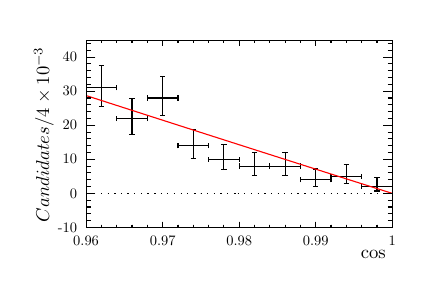
\begin{tikzpicture}
\pgfdeclareplotmark{cross} {
\pgfpathmoveto{\pgfpoint{-0.3\pgfplotmarksize}{\pgfplotmarksize}}
\pgfpathlineto{\pgfpoint{+0.3\pgfplotmarksize}{\pgfplotmarksize}}
\pgfpathlineto{\pgfpoint{+0.3\pgfplotmarksize}{0.3\pgfplotmarksize}}
\pgfpathlineto{\pgfpoint{+1\pgfplotmarksize}{0.3\pgfplotmarksize}}
\pgfpathlineto{\pgfpoint{+1\pgfplotmarksize}{-0.3\pgfplotmarksize}}
\pgfpathlineto{\pgfpoint{+0.3\pgfplotmarksize}{-0.3\pgfplotmarksize}}
\pgfpathlineto{\pgfpoint{+0.3\pgfplotmarksize}{-1.\pgfplotmarksize}}
\pgfpathlineto{\pgfpoint{-0.3\pgfplotmarksize}{-1.\pgfplotmarksize}}
\pgfpathlineto{\pgfpoint{-0.3\pgfplotmarksize}{-0.3\pgfplotmarksize}}
\pgfpathlineto{\pgfpoint{-1.\pgfplotmarksize}{-0.3\pgfplotmarksize}}
\pgfpathlineto{\pgfpoint{-1.\pgfplotmarksize}{0.3\pgfplotmarksize}}
\pgfpathlineto{\pgfpoint{-0.3\pgfplotmarksize}{0.3\pgfplotmarksize}}
\pgfpathclose
\pgfusepathqstroke
}
\pgfdeclareplotmark{cross*} {
\pgfpathmoveto{\pgfpoint{-0.3\pgfplotmarksize}{\pgfplotmarksize}}
\pgfpathlineto{\pgfpoint{+0.3\pgfplotmarksize}{\pgfplotmarksize}}
\pgfpathlineto{\pgfpoint{+0.3\pgfplotmarksize}{0.3\pgfplotmarksize}}
\pgfpathlineto{\pgfpoint{+1\pgfplotmarksize}{0.3\pgfplotmarksize}}
\pgfpathlineto{\pgfpoint{+1\pgfplotmarksize}{-0.3\pgfplotmarksize}}
\pgfpathlineto{\pgfpoint{+0.3\pgfplotmarksize}{-0.3\pgfplotmarksize}}
\pgfpathlineto{\pgfpoint{+0.3\pgfplotmarksize}{-1.\pgfplotmarksize}}
\pgfpathlineto{\pgfpoint{-0.3\pgfplotmarksize}{-1.\pgfplotmarksize}}
\pgfpathlineto{\pgfpoint{-0.3\pgfplotmarksize}{-0.3\pgfplotmarksize}}
\pgfpathlineto{\pgfpoint{-1.\pgfplotmarksize}{-0.3\pgfplotmarksize}}
\pgfpathlineto{\pgfpoint{-1.\pgfplotmarksize}{0.3\pgfplotmarksize}}
\pgfpathlineto{\pgfpoint{-0.3\pgfplotmarksize}{0.3\pgfplotmarksize}}
\pgfpathclose
\pgfusepathqfillstroke
}
\pgfdeclareplotmark{newstar} {
\pgfpathmoveto{\pgfqpoint{0pt}{\pgfplotmarksize}}
\pgfpathlineto{\pgfqpointpolar{44}{0.5\pgfplotmarksize}}
\pgfpathlineto{\pgfqpointpolar{18}{\pgfplotmarksize}}
\pgfpathlineto{\pgfqpointpolar{-20}{0.5\pgfplotmarksize}}
\pgfpathlineto{\pgfqpointpolar{-54}{\pgfplotmarksize}}
\pgfpathlineto{\pgfqpointpolar{-90}{0.5\pgfplotmarksize}}
\pgfpathlineto{\pgfqpointpolar{234}{\pgfplotmarksize}}
\pgfpathlineto{\pgfqpointpolar{198}{0.5\pgfplotmarksize}}
\pgfpathlineto{\pgfqpointpolar{162}{\pgfplotmarksize}}
\pgfpathlineto{\pgfqpointpolar{134}{0.5\pgfplotmarksize}}
\pgfpathclose
\pgfusepathqstroke
}
\pgfdeclareplotmark{newstar*} {
\pgfpathmoveto{\pgfqpoint{0pt}{\pgfplotmarksize}}
\pgfpathlineto{\pgfqpointpolar{44}{0.5\pgfplotmarksize}}
\pgfpathlineto{\pgfqpointpolar{18}{\pgfplotmarksize}}
\pgfpathlineto{\pgfqpointpolar{-20}{0.5\pgfplotmarksize}}
\pgfpathlineto{\pgfqpointpolar{-54}{\pgfplotmarksize}}
\pgfpathlineto{\pgfqpointpolar{-90}{0.5\pgfplotmarksize}}
\pgfpathlineto{\pgfqpointpolar{234}{\pgfplotmarksize}}
\pgfpathlineto{\pgfqpointpolar{198}{0.5\pgfplotmarksize}}
\pgfpathlineto{\pgfqpointpolar{162}{\pgfplotmarksize}}
\pgfpathlineto{\pgfqpointpolar{134}{0.5\pgfplotmarksize}}
\pgfpathclose
\pgfusepathqfillstroke
}
\definecolor{c}{rgb}{1,1,1};
\draw [color=c, fill=c] (0.1,3.20034) rectangle (4.9,6.21242);
\draw [color=c, fill=c] (0.772,3.68227) rectangle (4.66,6.06181);
\definecolor{c}{rgb}{0,0,0};
\draw [c] (0.772,3.68227) -- (0.772,6.06181) -- (4.66,6.06181) -- (4.66,3.68227) -- (0.772,3.68227);
\draw [c,line width=0.4] (0.772,3.68227) -- (4.66,3.68227);
\draw [anchor= east] (4.66,3.34492) node[scale=0.672711, rotate=0]{$\cos\thetaK$};
\draw [c,line width=0.4] (0.772,3.75546) -- (0.772,3.68227);
\draw [c,line width=0.4] (0.9664,3.71887) -- (0.9664,3.68227);
\draw [c,line width=0.4] (1.1608,3.71887) -- (1.1608,3.68227);
\draw [c,line width=0.4] (1.3552,3.71887) -- (1.3552,3.68227);
\draw [c,line width=0.4] (1.5496,3.71887) -- (1.5496,3.68227);
\draw [c,line width=0.4] (1.744,3.75546) -- (1.744,3.68227);
\draw [c,line width=0.4] (1.9384,3.71887) -- (1.9384,3.68227);
\draw [c,line width=0.4] (2.1328,3.71887) -- (2.1328,3.68227);
\draw [c,line width=0.4] (2.3272,3.71887) -- (2.3272,3.68227);
\draw [c,line width=0.4] (2.5216,3.71887) -- (2.5216,3.68227);
\draw [c,line width=0.4] (2.716,3.75546) -- (2.716,3.68227);
\draw [c,line width=0.4] (2.9104,3.71887) -- (2.9104,3.68227);
\draw [c,line width=0.4] (3.1048,3.71887) -- (3.1048,3.68227);
\draw [c,line width=0.4] (3.2992,3.71887) -- (3.2992,3.68227);
\draw [c,line width=0.4] (3.4936,3.71887) -- (3.4936,3.68227);
\draw [c,line width=0.4] (3.688,3.75546) -- (3.688,3.68227);
\draw [c,line width=0.4] (3.8824,3.71887) -- (3.8824,3.68227);
\draw [c,line width=0.4] (4.0768,3.71887) -- (4.0768,3.68227);
\draw [c,line width=0.4] (4.2712,3.71887) -- (4.2712,3.68227);
\draw [c,line width=0.4] (4.4656,3.71887) -- (4.4656,3.68227);
\draw [c,line width=0.4] (4.66,3.75546) -- (4.66,3.68227);
\draw [anchor=base] (0.772,3.45937) node[scale=0.52322, rotate=0]{0.96};
\draw [anchor=base] (1.744,3.45937) node[scale=0.52322, rotate=0]{0.97};
\draw [anchor=base] (2.716,3.45937) node[scale=0.52322, rotate=0]{0.98};
\draw [anchor=base] (3.688,3.45937) node[scale=0.52322, rotate=0]{0.99};
\draw [anchor=base] (4.66,3.45937) node[scale=0.52322, rotate=0]{1};
\draw [c,line width=0.4] (0.772,6.06181) -- (4.66,6.06181);
\draw [c,line width=0.4] (0.772,5.98862) -- (0.772,6.06181);
\draw [c,line width=0.4] (0.9664,6.02522) -- (0.9664,6.06181);
\draw [c,line width=0.4] (1.1608,6.02522) -- (1.1608,6.06181);
\draw [c,line width=0.4] (1.3552,6.02522) -- (1.3552,6.06181);
\draw [c,line width=0.4] (1.5496,6.02522) -- (1.5496,6.06181);
\draw [c,line width=0.4] (1.744,5.98862) -- (1.744,6.06181);
\draw [c,line width=0.4] (1.9384,6.02522) -- (1.9384,6.06181);
\draw [c,line width=0.4] (2.1328,6.02522) -- (2.1328,6.06181);
\draw [c,line width=0.4] (2.3272,6.02522) -- (2.3272,6.06181);
\draw [c,line width=0.4] (2.5216,6.02522) -- (2.5216,6.06181);
\draw [c,line width=0.4] (2.716,5.98862) -- (2.716,6.06181);
\draw [c,line width=0.4] (2.9104,6.02522) -- (2.9104,6.06181);
\draw [c,line width=0.4] (3.1048,6.02522) -- (3.1048,6.06181);
\draw [c,line width=0.4] (3.2992,6.02522) -- (3.2992,6.06181);
\draw [c,line width=0.4] (3.4936,6.02522) -- (3.4936,6.06181);
\draw [c,line width=0.4] (3.688,5.98862) -- (3.688,6.06181);
\draw [c,line width=0.4] (3.8824,6.02522) -- (3.8824,6.06181);
\draw [c,line width=0.4] (4.0768,6.02522) -- (4.0768,6.06181);
\draw [c,line width=0.4] (4.2712,6.02522) -- (4.2712,6.06181);
\draw [c,line width=0.4] (4.4656,6.02522) -- (4.4656,6.06181);
\draw [c,line width=0.4] (4.66,5.98862) -- (4.66,6.06181);
\draw [c,line width=0.4] (0.772,3.68227) -- (0.772,6.06181);
\draw [anchor= east] (0.2344,6.06181) node[scale=0.672711, rotate=90]{$\text{Candidates} / 4\times10^{-3}$};
\draw [c,line width=0.4] (0.88576,3.68227) -- (0.772,3.68227);
\draw [c,line width=0.4] (0.82888,3.7688) -- (0.772,3.7688);
\draw [c,line width=0.4] (0.82888,3.85533) -- (0.772,3.85533);
\draw [c,line width=0.4] (0.82888,3.94186) -- (0.772,3.94186);
\draw [c,line width=0.4] (0.82888,4.02838) -- (0.772,4.02838);
\draw [c,line width=0.4] (0.88576,4.11491) -- (0.772,4.11491);
\draw [c,line width=0.4] (0.82888,4.20144) -- (0.772,4.20144);
\draw [c,line width=0.4] (0.82888,4.28797) -- (0.772,4.28797);
\draw [c,line width=0.4] (0.82888,4.3745) -- (0.772,4.3745);
\draw [c,line width=0.4] (0.82888,4.46103) -- (0.772,4.46103);
\draw [c,line width=0.4] (0.88576,4.54756) -- (0.772,4.54756);
\draw [c,line width=0.4] (0.82888,4.63409) -- (0.772,4.63409);
\draw [c,line width=0.4] (0.82888,4.72061) -- (0.772,4.72061);
\draw [c,line width=0.4] (0.82888,4.80714) -- (0.772,4.80714);
\draw [c,line width=0.4] (0.82888,4.89367) -- (0.772,4.89367);
\draw [c,line width=0.4] (0.88576,4.9802) -- (0.772,4.9802);
\draw [c,line width=0.4] (0.82888,5.06673) -- (0.772,5.06673);
\draw [c,line width=0.4] (0.82888,5.15326) -- (0.772,5.15326);
\draw [c,line width=0.4] (0.82888,5.23979) -- (0.772,5.23979);
\draw [c,line width=0.4] (0.82888,5.32632) -- (0.772,5.32632);
\draw [c,line width=0.4] (0.88576,5.41285) -- (0.772,5.41285);
\draw [c,line width=0.4] (0.82888,5.49937) -- (0.772,5.49937);
\draw [c,line width=0.4] (0.82888,5.5859) -- (0.772,5.5859);
\draw [c,line width=0.4] (0.82888,5.67243) -- (0.772,5.67243);
\draw [c,line width=0.4] (0.82888,5.75896) -- (0.772,5.75896);
\draw [c,line width=0.4] (0.88576,5.84549) -- (0.772,5.84549);
\draw [c,line width=0.4] (0.88576,5.84549) -- (0.772,5.84549);
\draw [c,line width=0.4] (0.82888,5.93202) -- (0.772,5.93202);
\draw [c,line width=0.4] (0.82888,6.01855) -- (0.772,6.01855);
\draw [anchor= east] (0.724,3.68227) node[scale=0.52322, rotate=0]{-10};
\draw [anchor= east] (0.724,4.11491) node[scale=0.52322, rotate=0]{0};
\draw [anchor= east] (0.724,4.54756) node[scale=0.52322, rotate=0]{10};
\draw [anchor= east] (0.724,4.9802) node[scale=0.52322, rotate=0]{20};
\draw [anchor= east] (0.724,5.41285) node[scale=0.52322, rotate=0]{30};
\draw [anchor= east] (0.724,5.84549) node[scale=0.52322, rotate=0]{40};
\draw [c,line width=0.4] (4.66,3.68227) -- (4.66,6.06181);
\draw [c,line width=0.4] (4.54624,3.68227) -- (4.66,3.68227);
\draw [c,line width=0.4] (4.60312,3.7688) -- (4.66,3.7688);
\draw [c,line width=0.4] (4.60312,3.85533) -- (4.66,3.85533);
\draw [c,line width=0.4] (4.60312,3.94186) -- (4.66,3.94186);
\draw [c,line width=0.4] (4.60312,4.02838) -- (4.66,4.02838);
\draw [c,line width=0.4] (4.54624,4.11491) -- (4.66,4.11491);
\draw [c,line width=0.4] (4.60312,4.20144) -- (4.66,4.20144);
\draw [c,line width=0.4] (4.60312,4.28797) -- (4.66,4.28797);
\draw [c,line width=0.4] (4.60312,4.3745) -- (4.66,4.3745);
\draw [c,line width=0.4] (4.60312,4.46103) -- (4.66,4.46103);
\draw [c,line width=0.4] (4.54624,4.54756) -- (4.66,4.54756);
\draw [c,line width=0.4] (4.60312,4.63409) -- (4.66,4.63409);
\draw [c,line width=0.4] (4.60312,4.72061) -- (4.66,4.72061);
\draw [c,line width=0.4] (4.60312,4.80714) -- (4.66,4.80714);
\draw [c,line width=0.4] (4.60312,4.89367) -- (4.66,4.89367);
\draw [c,line width=0.4] (4.54624,4.9802) -- (4.66,4.9802);
\draw [c,line width=0.4] (4.60312,5.06673) -- (4.66,5.06673);
\draw [c,line width=0.4] (4.60312,5.15326) -- (4.66,5.15326);
\draw [c,line width=0.4] (4.60312,5.23979) -- (4.66,5.23979);
\draw [c,line width=0.4] (4.60312,5.32632) -- (4.66,5.32632);
\draw [c,line width=0.4] (4.54624,5.41285) -- (4.66,5.41285);
\draw [c,line width=0.4] (4.60312,5.49937) -- (4.66,5.49937);
\draw [c,line width=0.4] (4.60312,5.5859) -- (4.66,5.5859);
\draw [c,line width=0.4] (4.60312,5.67243) -- (4.66,5.67243);
\draw [c,line width=0.4] (4.60312,5.75896) -- (4.66,5.75896);
\draw [c,line width=0.4] (4.54624,5.84549) -- (4.66,5.84549);
\draw [c,line width=0.4] (4.54624,5.84549) -- (4.66,5.84549);
\draw [c,line width=0.4] (4.60312,5.93202) -- (4.66,5.93202);
\draw [c,line width=0.4] (4.60312,6.01855) -- (4.66,6.01855);
\draw [c,line width=0.4] (0.9664,5.45611) -- (0.772,5.45611);
\draw [c,line width=0.4] (0.772,5.42255) -- (0.772,5.48967);
\draw [c,line width=0.4] (0.9664,5.45611) -- (1.1608,5.45611);
\draw [c,line width=0.4] (1.1608,5.42255) -- (1.1608,5.48967);
\draw [c,line width=0.4] (0.9664,5.45611) -- (0.9664,5.74285);
\draw [c,line width=0.4] (0.932843,5.74285) -- (0.999957,5.74285);
\draw [c,line width=0.4] (0.9664,5.45611) -- (0.9664,5.21653);
\draw [c,line width=0.4] (0.932843,5.21653) -- (0.999957,5.21653);
\draw [c,line width=0.4] (1.3552,5.06673) -- (1.1608,5.06673);
\draw [c,line width=0.4] (1.1608,5.03317) -- (1.1608,5.10029);
\draw [c,line width=0.4] (1.3552,5.06673) -- (1.5496,5.06673);
\draw [c,line width=0.4] (1.5496,5.03317) -- (1.5496,5.10029);
\draw [c,line width=0.4] (1.3552,5.06673) -- (1.3552,5.31599);
\draw [c,line width=0.4] (1.32164,5.31599) -- (1.38876,5.31599);
\draw [c,line width=0.4] (1.3552,5.06673) -- (1.3552,4.86536);
\draw [c,line width=0.4] (1.32164,4.86536) -- (1.38876,4.86536);
\draw [c,line width=0.4] (1.744,5.32632) -- (1.5496,5.32632);
\draw [c,line width=0.4] (1.5496,5.29276) -- (1.5496,5.35987);
\draw [c,line width=0.4] (1.744,5.32632) -- (1.9384,5.32632);
\draw [c,line width=0.4] (1.9384,5.29276) -- (1.9384,5.35987);
\draw [c,line width=0.4] (1.744,5.32632) -- (1.744,5.60124);
\draw [c,line width=0.4] (1.71044,5.60124) -- (1.77756,5.60124);
\draw [c,line width=0.4] (1.744,5.32632) -- (1.744,5.09876);
\draw [c,line width=0.4] (1.71044,5.09876) -- (1.77756,5.09876);
\draw [c,line width=0.4] (2.1328,4.72061) -- (1.9384,4.72061);
\draw [c,line width=0.4] (1.9384,4.68706) -- (1.9384,4.75417);
\draw [c,line width=0.4] (2.1328,4.72061) -- (2.3272,4.72061);
\draw [c,line width=0.4] (2.3272,4.68706) -- (2.3272,4.75417);
\draw [c,line width=0.4] (2.1328,4.72061) -- (2.1328,4.9296);
\draw [c,line width=0.4] (2.09924,4.9296) -- (2.16636,4.9296);
\draw [c,line width=0.4] (2.1328,4.72061) -- (2.1328,4.56069);
\draw [c,line width=0.4] (2.09924,4.56069) -- (2.16636,4.56069);
\draw [c,line width=0.4] (2.5216,4.54756) -- (2.3272,4.54756);
\draw [c,line width=0.4] (2.3272,4.514) -- (2.3272,4.58111);
\draw [c,line width=0.4] (2.5216,4.54756) -- (2.716,4.54756);
\draw [c,line width=0.4] (2.716,4.514) -- (2.716,4.58111);
\draw [c,line width=0.4] (2.5216,4.54756) -- (2.5216,4.73216);
\draw [c,line width=0.4] (2.48804,4.73216) -- (2.55516,4.73216);
\draw [c,line width=0.4] (2.5216,4.54756) -- (2.5216,4.41306);
\draw [c,line width=0.4] (2.48804,4.41306) -- (2.55516,4.41306);
\draw [c,line width=0.4] (2.9104,4.46103) -- (2.716,4.46103);
\draw [c,line width=0.4] (2.716,4.42747) -- (2.716,4.49459);
\draw [c,line width=0.4] (2.9104,4.46103) -- (3.1048,4.46103);
\draw [c,line width=0.4] (3.1048,4.42747) -- (3.1048,4.49459);
\draw [c,line width=0.4] (2.9104,4.46103) -- (2.9104,4.63171);
\draw [c,line width=0.4] (2.87684,4.63171) -- (2.94396,4.63171);
\draw [c,line width=0.4] (2.9104,4.46103) -- (2.9104,4.34126);
\draw [c,line width=0.4] (2.87684,4.34126) -- (2.94396,4.34126);
\draw [c,line width=0.4] (3.2992,4.46103) -- (3.1048,4.46103);
\draw [c,line width=0.4] (3.1048,4.42747) -- (3.1048,4.49459);
\draw [c,line width=0.4] (3.2992,4.46103) -- (3.4936,4.46103);
\draw [c,line width=0.4] (3.4936,4.42747) -- (3.4936,4.49459);
\draw [c,line width=0.4] (3.2992,4.46103) -- (3.2992,4.63171);
\draw [c,line width=0.4] (3.26564,4.63171) -- (3.33276,4.63171);
\draw [c,line width=0.4] (3.2992,4.46103) -- (3.2992,4.34126);
\draw [c,line width=0.4] (3.26564,4.34126) -- (3.33276,4.34126);
\draw [c,line width=0.4] (3.688,4.28797) -- (3.4936,4.28797);
\draw [c,line width=0.4] (3.4936,4.25441) -- (3.4936,4.32153);
\draw [c,line width=0.4] (3.688,4.28797) -- (3.8824,4.28797);
\draw [c,line width=0.4] (3.8824,4.25441) -- (3.8824,4.32153);
\draw [c,line width=0.4] (3.688,4.28797) -- (3.688,4.42481);
\draw [c,line width=0.4] (3.65444,4.42481) -- (3.72156,4.42481);
\draw [c,line width=0.4] (3.688,4.28797) -- (3.688,4.20515);
\draw [c,line width=0.4] (3.65444,4.20515) -- (3.72156,4.20515);
\draw [c,line width=0.4] (4.0768,4.33123) -- (3.8824,4.33123);
\draw [c,line width=0.4] (3.8824,4.29768) -- (3.8824,4.36479);
\draw [c,line width=0.4] (4.0768,4.33123) -- (4.2712,4.33123);
\draw [c,line width=0.4] (4.2712,4.29768) -- (4.2712,4.36479);
\draw [c,line width=0.4] (4.0768,4.33123) -- (4.0768,4.47758);
\draw [c,line width=0.4] (4.04324,4.47758) -- (4.11036,4.47758);
\draw [c,line width=0.4] (4.0768,4.33123) -- (4.0768,4.2378);
\draw [c,line width=0.4] (4.04324,4.2378) -- (4.11036,4.2378);
\draw [c,line width=0.4] (4.4656,4.20144) -- (4.2712,4.20144);
\draw [c,line width=0.4] (4.2712,4.16788) -- (4.2712,4.235);
\draw [c,line width=0.4] (4.4656,4.20144) -- (4.66,4.20144);
\draw [c,line width=0.4] (4.66,4.16788) -- (4.66,4.235);
\draw [c,line width=0.4] (4.4656,4.20144) -- (4.4656,4.31557);
\draw [c,line width=0.4] (4.43204,4.31557) -- (4.49916,4.31557);
\draw [c,line width=0.4] (4.4656,4.20144) -- (4.4656,4.14555);
\draw [c,line width=0.4] (4.43204,4.14555) -- (4.49916,4.14555);
\foreach \P in {(0.9664,5.45611),(1.3552,5.06673),(1.744,5.32632),(2.1328,4.72061),(2.5216,4.54756),(2.9104,4.46103),(3.2992,4.46103),(3.688,4.28797),(4.0768,4.33123),(4.4656,4.20144)}{\draw[mark options={color=c,fill=c},mark size=0.960961pt,mark=]
 plot coordinates {\P};}
\definecolor{c}{rgb}{1,0,0};
\draw [c,line width=0.4] (0.772,5.35728) -- (0.772,5.35728);
\draw [c,line width=0.4] (0.772,5.35728) -- (1.1608,5.23202) -- (1.5496,5.1069) -- (1.9384,4.98194) -- (2.3272,4.85718) -- (2.716,4.73266) -- (3.1048,4.60841) -- (3.4936,4.48447) -- (3.8824,4.36088) -- (4.2712,4.23768) -- (4.66,4.11491) --
 (4.66,4.11491) -- (4.66,4.11491);
\definecolor{c}{rgb}{0,0,0};
\draw [c,line width=0.4] (0.772,3.68227) -- (4.66,3.68227);
\draw [c,line width=0.4] (0.772,3.75546) -- (0.772,3.68227);
\draw [c,line width=0.4] (0.9664,3.71887) -- (0.9664,3.68227);
\draw [c,line width=0.4] (1.1608,3.71887) -- (1.1608,3.68227);
\draw [c,line width=0.4] (1.3552,3.71887) -- (1.3552,3.68227);
\draw [c,line width=0.4] (1.5496,3.71887) -- (1.5496,3.68227);
\draw [c,line width=0.4] (1.744,3.75546) -- (1.744,3.68227);
\draw [c,line width=0.4] (1.9384,3.71887) -- (1.9384,3.68227);
\draw [c,line width=0.4] (2.1328,3.71887) -- (2.1328,3.68227);
\draw [c,line width=0.4] (2.3272,3.71887) -- (2.3272,3.68227);
\draw [c,line width=0.4] (2.5216,3.71887) -- (2.5216,3.68227);
\draw [c,line width=0.4] (2.716,3.75546) -- (2.716,3.68227);
\draw [c,line width=0.4] (2.9104,3.71887) -- (2.9104,3.68227);
\draw [c,line width=0.4] (3.1048,3.71887) -- (3.1048,3.68227);
\draw [c,line width=0.4] (3.2992,3.71887) -- (3.2992,3.68227);
\draw [c,line width=0.4] (3.4936,3.71887) -- (3.4936,3.68227);
\draw [c,line width=0.4] (3.688,3.75546) -- (3.688,3.68227);
\draw [c,line width=0.4] (3.8824,3.71887) -- (3.8824,3.68227);
\draw [c,line width=0.4] (4.0768,3.71887) -- (4.0768,3.68227);
\draw [c,line width=0.4] (4.2712,3.71887) -- (4.2712,3.68227);
\draw [c,line width=0.4] (4.4656,3.71887) -- (4.4656,3.68227);
\draw [c,line width=0.4] (4.66,3.75546) -- (4.66,3.68227);
\draw [c,line width=0.4] (0.772,6.06181) -- (4.66,6.06181);
\draw [c,line width=0.4] (0.772,5.98862) -- (0.772,6.06181);
\draw [c,line width=0.4] (0.9664,6.02522) -- (0.9664,6.06181);
\draw [c,line width=0.4] (1.1608,6.02522) -- (1.1608,6.06181);
\draw [c,line width=0.4] (1.3552,6.02522) -- (1.3552,6.06181);
\draw [c,line width=0.4] (1.5496,6.02522) -- (1.5496,6.06181);
\draw [c,line width=0.4] (1.744,5.98862) -- (1.744,6.06181);
\draw [c,line width=0.4] (1.9384,6.02522) -- (1.9384,6.06181);
\draw [c,line width=0.4] (2.1328,6.02522) -- (2.1328,6.06181);
\draw [c,line width=0.4] (2.3272,6.02522) -- (2.3272,6.06181);
\draw [c,line width=0.4] (2.5216,6.02522) -- (2.5216,6.06181);
\draw [c,line width=0.4] (2.716,5.98862) -- (2.716,6.06181);
\draw [c,line width=0.4] (2.9104,6.02522) -- (2.9104,6.06181);
\draw [c,line width=0.4] (3.1048,6.02522) -- (3.1048,6.06181);
\draw [c,line width=0.4] (3.2992,6.02522) -- (3.2992,6.06181);
\draw [c,line width=0.4] (3.4936,6.02522) -- (3.4936,6.06181);
\draw [c,line width=0.4] (3.688,5.98862) -- (3.688,6.06181);
\draw [c,line width=0.4] (3.8824,6.02522) -- (3.8824,6.06181);
\draw [c,line width=0.4] (4.0768,6.02522) -- (4.0768,6.06181);
\draw [c,line width=0.4] (4.2712,6.02522) -- (4.2712,6.06181);
\draw [c,line width=0.4] (4.4656,6.02522) -- (4.4656,6.06181);
\draw [c,line width=0.4] (4.66,5.98862) -- (4.66,6.06181);
\draw [c,line width=0.4] (0.772,3.68227) -- (0.772,6.06181);
\draw [c,line width=0.4] (0.88576,3.68227) -- (0.772,3.68227);
\draw [c,line width=0.4] (0.82888,3.7688) -- (0.772,3.7688);
\draw [c,line width=0.4] (0.82888,3.85533) -- (0.772,3.85533);
\draw [c,line width=0.4] (0.82888,3.94186) -- (0.772,3.94186);
\draw [c,line width=0.4] (0.82888,4.02838) -- (0.772,4.02838);
\draw [c,line width=0.4] (0.88576,4.11491) -- (0.772,4.11491);
\draw [c,line width=0.4] (0.82888,4.20144) -- (0.772,4.20144);
\draw [c,line width=0.4] (0.82888,4.28797) -- (0.772,4.28797);
\draw [c,line width=0.4] (0.82888,4.3745) -- (0.772,4.3745);
\draw [c,line width=0.4] (0.82888,4.46103) -- (0.772,4.46103);
\draw [c,line width=0.4] (0.88576,4.54756) -- (0.772,4.54756);
\draw [c,line width=0.4] (0.82888,4.63409) -- (0.772,4.63409);
\draw [c,line width=0.4] (0.82888,4.72061) -- (0.772,4.72061);
\draw [c,line width=0.4] (0.82888,4.80714) -- (0.772,4.80714);
\draw [c,line width=0.4] (0.82888,4.89367) -- (0.772,4.89367);
\draw [c,line width=0.4] (0.88576,4.9802) -- (0.772,4.9802);
\draw [c,line width=0.4] (0.82888,5.06673) -- (0.772,5.06673);
\draw [c,line width=0.4] (0.82888,5.15326) -- (0.772,5.15326);
\draw [c,line width=0.4] (0.82888,5.23979) -- (0.772,5.23979);
\draw [c,line width=0.4] (0.82888,5.32632) -- (0.772,5.32632);
\draw [c,line width=0.4] (0.88576,5.41285) -- (0.772,5.41285);
\draw [c,line width=0.4] (0.82888,5.49937) -- (0.772,5.49937);
\draw [c,line width=0.4] (0.82888,5.5859) -- (0.772,5.5859);
\draw [c,line width=0.4] (0.82888,5.67243) -- (0.772,5.67243);
\draw [c,line width=0.4] (0.82888,5.75896) -- (0.772,5.75896);
\draw [c,line width=0.4] (0.88576,5.84549) -- (0.772,5.84549);
\draw [c,line width=0.4] (0.88576,5.84549) -- (0.772,5.84549);
\draw [c,line width=0.4] (0.82888,5.93202) -- (0.772,5.93202);
\draw [c,line width=0.4] (0.82888,6.01855) -- (0.772,6.01855);
\draw [c,line width=0.4] (4.66,3.68227) -- (4.66,6.06181);
\draw [c,line width=0.4] (4.54624,3.68227) -- (4.66,3.68227);
\draw [c,line width=0.4] (4.60312,3.7688) -- (4.66,3.7688);
\draw [c,line width=0.4] (4.60312,3.85533) -- (4.66,3.85533);
\draw [c,line width=0.4] (4.60312,3.94186) -- (4.66,3.94186);
\draw [c,line width=0.4] (4.60312,4.02838) -- (4.66,4.02838);
\draw [c,line width=0.4] (4.54624,4.11491) -- (4.66,4.11491);
\draw [c,line width=0.4] (4.60312,4.20144) -- (4.66,4.20144);
\draw [c,line width=0.4] (4.60312,4.28797) -- (4.66,4.28797);
\draw [c,line width=0.4] (4.60312,4.3745) -- (4.66,4.3745);
\draw [c,line width=0.4] (4.60312,4.46103) -- (4.66,4.46103);
\draw [c,line width=0.4] (4.54624,4.54756) -- (4.66,4.54756);
\draw [c,line width=0.4] (4.60312,4.63409) -- (4.66,4.63409);
\draw [c,line width=0.4] (4.60312,4.72061) -- (4.66,4.72061);
\draw [c,line width=0.4] (4.60312,4.80714) -- (4.66,4.80714);
\draw [c,line width=0.4] (4.60312,4.89367) -- (4.66,4.89367);
\draw [c,line width=0.4] (4.54624,4.9802) -- (4.66,4.9802);
\draw [c,line width=0.4] (4.60312,5.06673) -- (4.66,5.06673);
\draw [c,line width=0.4] (4.60312,5.15326) -- (4.66,5.15326);
\draw [c,line width=0.4] (4.60312,5.23979) -- (4.66,5.23979);
\draw [c,line width=0.4] (4.60312,5.32632) -- (4.66,5.32632);
\draw [c,line width=0.4] (4.54624,5.41285) -- (4.66,5.41285);
\draw [c,line width=0.4] (4.60312,5.49937) -- (4.66,5.49937);
\draw [c,line width=0.4] (4.60312,5.5859) -- (4.66,5.5859);
\draw [c,line width=0.4] (4.60312,5.67243) -- (4.66,5.67243);
\draw [c,line width=0.4] (4.60312,5.75896) -- (4.66,5.75896);
\draw [c,line width=0.4] (4.54624,5.84549) -- (4.66,5.84549);
\draw [c,line width=0.4] (4.54624,5.84549) -- (4.66,5.84549);
\draw [c,line width=0.4] (4.60312,5.93202) -- (4.66,5.93202);
\draw [c,line width=0.4] (4.60312,6.01855) -- (4.66,6.01855);
\draw [c,dotted,line width=0.4] (0.79144,4.11491) -- (0.83032,4.11491) -- (0.8692,4.11491) -- (0.90808,4.11491) -- (0.94696,4.11491) -- (0.98584,4.11491) -- (1.02472,4.11491) -- (1.0636,4.11491) -- (1.10248,4.11491) -- (1.14136,4.11491) --
 (1.18024,4.11491) -- (1.21912,4.11491) -- (1.258,4.11491) -- (1.29688,4.11491) -- (1.33576,4.11491) -- (1.37464,4.11491) -- (1.41352,4.11491) -- (1.4524,4.11491) -- (1.49128,4.11491) -- (1.53016,4.11491) -- (1.56904,4.11491) -- (1.60792,4.11491) --
 (1.6468,4.11491) -- (1.68568,4.11491) -- (1.72456,4.11491) -- (1.76344,4.11491) -- (1.80232,4.11491) -- (1.8412,4.11491) -- (1.88008,4.11491) -- (1.91896,4.11491) -- (1.95784,4.11491) -- (1.99672,4.11491) -- (2.0356,4.11491) -- (2.07448,4.11491) --
 (2.11336,4.11491) -- (2.15224,4.11491) -- (2.19112,4.11491) -- (2.23,4.11491) -- (2.26888,4.11491) -- (2.30776,4.11491) -- (2.34664,4.11491) -- (2.38552,4.11491) -- (2.4244,4.11491) -- (2.46328,4.11491) -- (2.50216,4.11491) -- (2.54104,4.11491) --
 (2.57992,4.11491) -- (2.6188,4.11491) -- (2.65768,4.11491) -- (2.69656,4.11491);
\draw [c,dotted,line width=0.4] (2.69656,4.11491) -- (2.73544,4.11491) -- (2.77432,4.11491) -- (2.8132,4.11491) -- (2.85208,4.11491) -- (2.89096,4.11491) -- (2.92984,4.11491) -- (2.96872,4.11491) -- (3.0076,4.11491) -- (3.04648,4.11491) --
 (3.08536,4.11491) -- (3.12424,4.11491) -- (3.16312,4.11491) -- (3.202,4.11491) -- (3.24088,4.11491) -- (3.27976,4.11491) -- (3.31864,4.11491) -- (3.35752,4.11491) -- (3.3964,4.11491) -- (3.43528,4.11491) -- (3.47416,4.11491) -- (3.51304,4.11491) --
 (3.55192,4.11491) -- (3.5908,4.11491) -- (3.62968,4.11491) -- (3.66856,4.11491) -- (3.70744,4.11491) -- (3.74632,4.11491) -- (3.7852,4.11491) -- (3.82408,4.11491) -- (3.86296,4.11491) -- (3.90184,4.11491) -- (3.94072,4.11491) -- (3.9796,4.11491) --
 (4.01848,4.11491) -- (4.05736,4.11491) -- (4.09624,4.11491) -- (4.13512,4.11491) -- (4.174,4.11491) -- (4.21288,4.11491) -- (4.25176,4.11491) -- (4.29064,4.11491) -- (4.32952,4.11491) -- (4.3684,4.11491) -- (4.40728,4.11491) -- (4.44616,4.11491) --
 (4.48504,4.11491) -- (4.52392,4.11491) -- (4.5628,4.11491) -- (4.60168,4.11491);
\draw [c,dotted,line width=0.4] (4.60168,4.11491) -- (4.64056,4.11491);
\end{tikzpicture}
}
    \caption{}
    % \label{angAcc_constr_fit}
  \end{subfigure}
  %% \begin{subfigure}{0.5\textwidth}
  %%   \tikzsetnextfilename{eff_helcosthetaK_neg_all_constr_zoom}
  %%   \scalebox{1.3}{\input{Figures/Chapter4/eff_helcosthetaK_neg_all_constr_zoom}}
  %%   \caption{}
  %%   \label{angAcc_constr}
  %% \end{subfigure}
  \caption{Angular \pdf projection corrected with the angular efficiency function before (A) and ater (B) constraining its value at $\cos\thetaK=1$ (red curve). 
           on top of the $\cos\thetaK$ distribution in the simulated sample (black points).
            }
  \label{angAcc_constr}
\end{figure}

Before laying out the formulas behind the above mentioned steps it is usefull to literally see the problem caused by the parametrization, see \figref{angAcc_nom}, \figref{angAcc_constr}
and the corresponding caption. Having done that the most natural thing to do before making any efford to force the value of \equref{eff_func}, hearafter efficiency function,
positive at $\cos\thetaK=1$ is to make the best choice of effiency moments. The moments are chosen such that the value of the efficiency function is as ``less negative``
as 
possible\footnote{It is actually not trivial to find a good choice of efficiecy moments. Two things are relevant when trying to describe a 
distribution with orthogonal functions like $P$ and $Y$. One is the shape of the orthogonal function itself and two the sign and size of the calculated moment.
For example the efficiency term $\moment{1}{0}{0}P_1Y_{00}$ is necessay to describe the drop of efficiency in $\cos\thetaK$ but the size of $\moment{1}{0}{0}$ 
is too large making the total efficiency function negative. Thus one could add the term $P_3Y_{00}\moment{3}{0}{0}$ where $\moment{3}{0}{0}$ is positive
(see \tabref{eff_moms_table} ) to counter the large negative value of $\moment{1}{0}{0}$ but unfortunatelly it is not enough. Things get more complicated
when trying to choose efficiency moments that affect the acceptance shape in all of its three domensions at the same time.
}.

Having chosen the best possible set of efficiency moments the value of the efficiency function is constrained by solving it for
one of the efficiency moments, which can be easily done for $\moment{0}{0}{0}$. The constrain that is imposed is shown in \equref{eff_func_constr}

\begin{center}
\begin{equation}
  \epsilon(\cos\thetaK = 1, \cos\thetamu, \phihel) = 0 
  \label{eff_func_constr}
\end{equation}
\end{center}

\noindent Starting from the efficiency function of \equref{eff_func} (where the sum now runs over the indices of the first column in \tabref{eff_moms_table}):

\begin{center}
\begin{align}
  \epsilon(\Omega) =& \sum_{ijk} \; c^i_{jk} \legendre{i}{0} \spharm{j}{k} \nonumber \\
                   =& \moment{0}{0}{0} \legendre{0}{0} \spharm{0}{0} + \sum_{ijk}^{ijk\neq 000} \; \moment{i}{j}{k} \legendre{i}{0} \spharm{j}{k}
  \label{eff_func_rewriten}
\end{align}
\end{center}

\noindent given \equref{eff_func_constr} and also $P_{0}^{0}=1$,  $Y_{00} = \frac{1}{2\sqrt{\pi}}$ \equref{eff_func_rewriten} can be 
easily solved for $\moment{0}{0}{0}$ resulting in \equref{eff_constr_mom}

\begin{center}
\begin{equation}
  \moment{0}{0}{0} = -2\sqrt{\pi} \sum_{ijk}^{ijk\neq 000} \; \moment{i}{j}{k} P_i^0(1) \spharm{j}{k}
  \label{eff_constr_mom}
\end{equation}
\end{center}

\noindent \equref{eff_func_rewriten} is used along with \equref{eff_constr_mom} resulting finally in \equref{eff_func_final}. 
The last is an updated efficiency function which is guranteed to be positive definite at $\cos\thetaK=1$. 

\begin{center}
\begin{align}
  \epsilon(\Omega) &= \left[-2\sqrt{\pi} \sum_{ijk}^{ijk\neq 000} \; \moment{i}{j}{k} \cancelto{1}{P_i^0(1)} \spharm{j}{k} \right] \cancelto{1}{\legendre{0}{0}} \cancelto{\frac{1}{2\sqrt{\pi}}}{\spharm{0}{0}} \nonumber \\ 
                   &+ \sum_{ijk}^{ijk\neq 000} \; \moment{i}{j}{k} \legendre{i}{0} \spharm{j}{k} = \nonumber \\
                   &= \left[- \sum_{ijk}^{ijk\neq 000} \; \moment{i}{j}{k} \spharm{j}{k} \right] + \sum_{ijk}^{ijk\neq 000} \; \moment{i}{j}{k} \legendre{i}{0} \spharm{j}{k} = \nonumber\\
                   &= \sum_{ijk}^{ijk\neq 000} \moment{i}{j}{k} \left[ \legendre{i}{0} \spharm{j}{k} - \spharm{j}{k} \right]
  \label{eff_func_final}
\end{align}
\end{center}

\noindent The result of the above constrain is shown in figure \figref{angAcc_constr}, where it can be seen that the acceptance projecton on $\cos\thetaK=1$
is not zero anymore. In addition it has also been checked wheather the acceptance is negative in 2D and 3D, since it is possible for a 2D
projetion of the acceptance to take negative values as well while the 1D projections are positive. Two dimentional preojection of the constrained acceptance can be seen in \figref{eff2D}.

Constraining the acceptance in this maner described above comes with a penalty, meaning that the shape of the 1D acceptance
projections is distorted a bit. In order to undo this distortion and describe better the acceptance shape an addional step is implemented. 
As it was previously mentioned the acceptance function of \equref{eff_func_final} is further fitted to the simulated data where the efficiency
moments are allowed to float with gaussian constraints of one standard deviation and properly taking into account their correlations by
means of a multivariant gaussian constrain. The fitting \pdf $\mathcal{P}= \Pgen \times\epsilon(\Omega;\vec{\bf c}) \times G(\vec{\bf{c}})$ 
consists of the \pdf that the simulated data was generated with multipied with the efficiency function \eqref{eff_func_final}. 
The generated parameters are fixed so that only the efficiecny moments are allowed to float.     
The multivariate gaussian function $G(\vec{\bf{c}})$, used to constrain the efficiency moments within one standard deviation is shown in \equref{mvm_constr}.

\begin{center}
\begin{equation}
  G(\vec{\bf{c}}) = \frac{1}{\sqrt{(2\pi)^k}|C|} \; e^{-\frac{1}{2}(  \vec{\bf{c}} - <{\bf{c}}>  )^{\text{T}} C^{-1} (\vec{\bf{c}} - <{\bf{c}}> ) }
  \label{mvm_constr}
\end{equation}
\end{center}

\noindent Where $\vec{\bf c}$ represents the floatting efficiency moments, whereas $<\vec{\bf c}>$ are the efficiency moments computed
with \equref{eff_constr_mom}. $C$ and $|C|$ are the covariance matrix of the efficiency moments and its determinant respectivelly.
Lastly $k$ is the number of efficiency moments present in \equref{eff_func_final}. 

\begin{figure}[h]
  \centering
  \begin{subfigure}{0.5\textwidth}
    \includegraphics[width=\textwidth]{Figures/Chapter4/canv_cosThK_cosThL_Sim08_3fb_hel_negKaons_all.pdf}
    \caption{}
    \label{eff2D_kl}
  \end{subfigure}%
  \hfill%
  \begin{subfigure}{0.5\textwidth}
    \includegraphics[width=\textwidth]{Figures/Chapter4/canv_cosThK_phi_Sim08_3fb_hel_negKaons_all.pdf}
    \caption{}
    \label{eff2D_kp}
  \end{subfigure}
  \begin{subfigure}{0.5\textwidth}
    \includegraphics[width=\textwidth]{Figures/Chapter4/canv_cosThL_phi_Sim08_3fb_hel_negKaons_all.pdf}
    \caption{}
    \label{eff2D_lp}
  \end{subfigure}
\caption{Two dimensional projections of the efficiency (after the constrain of \equref{eff_func_constr}).}
    \label{eff2D}
\end{figure}


\subsubsection{Alternative parameterization}
As it was mentioned before there is at least one more way to parametrize the angular acceptance, namely the \emph{normalization weights}.
The main difference between this aproach and the method adopted in this analysis is that essentially the normalization weights use the angular functions
of \tabref{ang_distr} as a basis to project the efficiency of \equref{eff_def}, instead of the orthogonal basis $a_i^{jk}$ of \equref{eff_func}.
Looking at \equref{norm_weights_pdf} it is helpfull to realise how the normalization weights, $\xi_n$, are introduced into the fitting \pdf. 
One can see that they effectivelly do not multiply the angular \pdf directly but modify the relative contributions between the angular functions
$f_n$, in the normalization integral of the fitting \pdf. The normalization weights are also calculated following the concept of Monte Carlo integration
similarly to the case of efficiency moments.

\begin{equation}
  \mathcal{P} \propto \frac{\sum_n f_k(\Omega)}{\sum_n \int d\Omega \; \epsilon(\Omega) \; f_k(\Omega)}, \;\;\;\;\text{where} \int d\Omega \; \epsilon(\Omega) \; f_k(\Omega) \equiv \xi_n 
  \label{norm_weights_pdf}
\end{equation}

The advantages of this method is that it is immune from any issue with negative efficiency values. After all the acceptance shape is not parametrised at all.
On the other hand the fitting time increases due to the fact that the \pdf is not expressed in an orthogonal basis any more. Also other
implementation and plotting issues arise when usign normalization weights. Lastly the two methods can give identical values on the fitted parameters by mapping 
the normalization weights to efficiency moments. This can be done if one solves the nornalization intregral, $\int d\Omega\;\Pgen\times\epsilon(\Omega)$
of the \pdf of \tabref{ang_distr} and the efficiency function in \equref{eff_func}, then the mapping of $\moment{i}{j}{k} \rightarrow \xi_n$ follos naturally
by expoliting the orthogonality of $P$ and $Y$. More details on the normalization weights aproach can be found in \cite{jeroenThesis}. 

%%%%%%%%%%%%%%%%%%%%%%%%%%%%%%%%%%%%%%%%%%%%%%%%
\subsection{Acceptance Corrections}
\label{Accceptance_Corrections}
%%%%%%%%%%%%%%%%%%%%%%%%%%%%%%%%%%%%%%%%%%%%%%%%
As it was mentioned in section \secref{Accceptance} the angular acceptance is determined with simulated \BsJpsiKst events.
Thus the acceptance determination can be trusted only if the simulation accurately describes the detector as well as the 
physical amplitudes of the \BsJpsiKst decay. More specifically real data - Mont Carlo differences in the momentum distributions
of the final state particles (\figref{} {\color{red} Make data-MC plots}) may reflect a different acceptance in data compared to MC. On the other hand,
non perfect acceptance simulation could be also atributed to differences in the underlying physical parameter values generating 
the Monte Carlo data and those present on real data. For example, the presence of S-wave in the real data (and its absence on simulated data)
can cause a difference in the observed kaon momentum spectrum even though the angular acceptance may be perfectly simulated.
Both of the above mentioned effects have an impact on the decay angles distribution since the helicity angles are defined
from the momenta of the final state particles. 

In order to over-come the problem of simulation imperfections, the simulated sample is weighted using an iterative procedure. 
At each weighting step of the procedure the Monte Carlo data are corrected for the current best estimate of the physics 
parameters and the two dimensional $p_{K^{\pm}},p_{\pi^{\mp}}$ momentum distribution. 
The efficiency moments are re-evaluated using the weighted Monte Carlo sample and the fit to the real data is repeated. 
This changes the best estimate of the physical parameters of interest. This procedure is reapetated untill the parameters
of interest converge. The full procedure by steps can be summarized as:

\begin{enumerate}
\item Calculate an initial set of efficiency moments using uncorrected \BsJpsiKst Monte Carlo samples.
\item Perform a fit on the \BsJpsiKst data using the initial eficiency moments, and obtain the first estimate of the physical parameters.
\item Weight each Monte Carlo event for the difference between the obtained from the previous fit angular PDF and the angular PDF used to generate the Monte Carlo sample. 
      This essentially means that the underlying physics of the reweighted Monte Carlo sample corresponds to the physics obtained in the previous step.
\item Compare the $p_{K^{\pm}},p_{\pi^{\mp}}$ momentum distribution between the physics weighted Monte Carlo sample of the previous step with the 
      real data, and weight again each Monte Carlo event for the difference.
\item Re-estimate the efficiency moments using the physics plus momentum corrected \BsJpsiKst Monte Carlo sample and repeat the fit to \BsJpsiKst data.
\item Go back to step 4 and repeat until change in the parameters of intereset are negligible ($<0.01\sigma$).
\end{enumerate} 

The $p_{K^{\pm}},p_{\pi^{\mp}}$ weighting of the MC sample is done using 2D histograms, with a binning scheme that is shown in \tabref{angAccBinning}. 
At least 5 iterations are necessary for convergence. Detailed evolution of the efficiency moments and the physics result after each iteration
can be found in \appref{}. In \tabref{} and \figref{} it can also be seen that the effect of the acceptance correction is small. {\color{red}Those tables
and plots will be added after I re-run the acceptance. They ofer little information for the effort they require to make }

\begin{table}[!h]
  \center
  \caption{\small Binning scheme for each of the re weighted variables. Bins have equal width.}
  \begin{tabular}{c c c}
    \hline
     variables & range & $\# \text{bins}$ \\
     %\multicolumn{2}{c}{range}   &  vs        \\
    \hline
    $p_{K^{\pm}}$    &  $[0,140]    \;  \text{GeV}/\text{c}^2$  & 10      \\ 
    $p_{\pi^{\pm}}$  &  $[0,60]      \;  \text{GeV}/\text{c}^2$  & 10      \\ 
   % $p(\Bs)$    &  $[x,y]   \;  \text{MeV}/\text{c}^2$  & 200      \\
   % \mkpi       &  $[x,y] \; \text{MeV}/\text{c}$    & 100      \\
    \hline
  \end{tabular}
  \label{angAccBinning}
\end{table}


\subsubsection{Validation of the iterative procedure}
{\color{red} The code for that is half implemented.}

%%%%%%%%%%%%%%%%%%%%%%%%%%%%%%%%%%%%%%%%%%%%%%%%
\subsection{\Kpi Invariant mass}
\label{Kpi_Invariant_mass}
%%%%%%%%%%%%%%%%%%%%%%%%%%%%%%%%%%%%%%%%%%%%%%%%

\subsubsection{Dependence on \mkpi and CSP factors}
The dependence of the \BJpsiKpi decay amplitude on \mkpi as it was introduced in \equref{ang_terms} is treated in a special way.
The $\mKpiAmp$ functions are not implemented but they are integrated over \mkpi instead while the fitting real data sample is binned in four parts.
Where in each part the \mkpi lineshape is ashumed to be flat.
The choice of this strategy is good enough given the fact that the \mkpi region relevant for this analysis is dominated by the well
known \pwave. Thus, developing a full mdoel for the both the \pwave and \swave is not the first priority in this analysis.

Despite the \mkpi integration there is still some residual dependence left. It originates from integrals
like the one in equation \equref{spIntegrals}

\begin{equation}
  \label{spIntegrals}
  \int d\mkpi \; \Phi \; \mKpiAmp^* \mKpiAmp[m]
\end{equation}

\noindent where $\mKpiAmp[n,m]$ run in the same way as in \equref{ang_terms} and $\Phi$ is a pahase space 
factor\footnote{$\Phi = \left[ \lambda(m_\mu,m_\kaon,m_\pion) \lambda(m_{\Bs},m_\jpsi,m_\mu) \right] / \; 4 m_\mu^2$  and \\ 
$\lambda(m_1,m_2,m_3) = \left[ m_1^2 - 2m_1^2(m_2^2 + m_3^2) + m_2^2 + m_3^2 - 2m_2^2m_3^2 \right] / m_1^2 $  
} and it eventually manifests only in the \spwave interference terms of table \tabref{eff_moms_table} as shown
in \equref{csp_def}.

\begin{equation}
  \label{csp_def}
  \frac{\int_{\mkpi^-}^{\mkpi^+} d\mkpi \; \Phi \; s^* \times p} {\int_{\mkpi^-}^{\mkpi^+} d\mkpi \; \Phi \; |s|^2 \; \int_{\mkpi^-}^{\mkpi^+} d\mkpi \; \Phi |p|^2} = \CSP \; e^{-i\ThetaSP} \ ,
\end{equation}

\noindent where $s$ and $p$ stand for the \swave and \pwave lineshapes respectivelly. Evaluating those complex valued integrals yield 
the so called $\CSP$ factors which are inserted in the angular functions of \tabref{ang_distr}. Particularly the real part is inserted
as a multiplicative factor in front of all \spwave interference
terms\footnote{for example $\ReAmp{0}{S} \rightarrow \CSP * \ReAmp{0}{S} $}.
Whereas the imaginary part, is absorbed by the phase difference of the same interference 
terms\footnote{ $\arg(A_0^*A_S) \rightarrow \arg(A_0^*A_S) - \ThetaSP$}. Floating the $\CSP$ factors in the fit is not prefared due
to high correlations with the decay amplitudes. Instead it would be better to extend the angular fit so that the \mkpi dependence 
is modeled directly via the $\mKpiAmp$ terms of \equref{ang_terms}. The above mentioned lineshapes that are necessary
to compute the $\CSP$ factors are a Isobar combination of a \KstENT and \KstOFOZ for $p$ and a LASS parametrization of a \KstOFTZ
with a non resonant term. LASS is a common \swave prametrization in amplitude analysis, it is a combination of a relativistic Breit-Wigner
with angular momentum barier factors. Whereas a Isobar is a superposition of resonances.


\subsubsection{sWeighted \mkpi distribution}
While the \Bs and \Bd di-muon sWeighted distributions have very similar shape, the \mkpi spectrums exhibit different shapes. 
Indeed, the \Bs \mkpi \sPlot seems to be slightly distorted, \figref{mkpiPlot_raw}. Since there is no reason why the \Kst$~$\pwave 
sould have different shape between \BsJpsiKst and \BdJpsiKst. This could be due to the presence of interference between
the $K\pi$ \swave and the \Kstarz, which may be stronger in the \Bs decays compared to the \Bd ones. In order 
to check the validity of this hypothesis, two additional studies are performed. First it was checked that the peaking
background treatment propagated to the \sWeights was not responsible for this behavior. Indeed, no significant difference 
between the \Bs \mkpi spectrum using \sWeights computed with and without Monte Carlo data injection was found. Second the \mkpi 
distribution is corrected for angular efficiency effects. This way the interference between the $K\pi$ \swave and the 
\Kstarz $ $ \pwave vanishes. This happens because for a perfect acceptance the interference terms in \tabref{ang_terms} integrated over all angles
evaluate to zero. Which is exactly what is shown in \figref{mkpiPlot_eff}. The \Bs \mkpi distribution is closer to the one of the \Bd after applying
the efficiency correction. This is a clear indication of the presence of stronger interference in the \Bs case compared to the \Bd one.

\begin{figure}[h]
  \centering
  \begin{subfigure}{0.5\textwidth}
    \tikzsetnextfilename{mKpi_raw}
    \scalebox{0.65}{\input{Figures/Chapter4/mKpi_raw}}
    \caption{}
    \label{mkpiPlot_raw}
  \end{subfigure}%
  \hfill%
  \begin{subfigure}{0.5\textwidth}
    \tikzsetnextfilename{mKpi_eff}
    \scalebox{0.65}{\input{Figures/Chapter4/mKpi_eff}}
    \caption{}
    \label{mkpiPlot_eff}
  \end{subfigure}
  \begin{subfigure}{0.5\textwidth}
    % \tikzsetnextfilename{mJpsi_eff} 
    %\scalebox{0.65}{\input{Figures/Chapter4/mJpsi_eff}}
    \caption{\color{red} sWeighted Jpsi mass here soon}
    \label{jpsiPlot}
  \end{subfigure}
\caption{sWeighted plots of \mkpi(top row) and \jpsi (bottom row). In the top right plot the \mkpi distribution
         is corrected for angular acceptance effects. This is done by weighting each event further with the inverse 
         of the acceptance function as obtained in \equref{eff_func_final}.}
\end{figure}

%%%%%%%%%%%%%%%%%%%%%%%%%%%%%%%%%%%%%%%%%%%%%%%%
\subsection{Production and Detection Assymetries}
\label{experimentalAssym}
%%%%%%%%%%%%%%%%%%%%%%%%%%%%%%%%%%%%%%%%%%%%%%%%
The nature of the current analysis is such that it is affected by assymetries releated to experimental effects.
This is intuitive considering the $\Acp{}$ parameter of intereset. As explained in \secref{TheBsJpsiKstDecay}
the last quantifies if the decay \BsJpsiKst takes place more often that its charge conjugate. Now in case the
colisions at \lhc favour one over the other or the detector has different efficiency for positive and negative 
kaons (or pions) then the $\Acp{}$ assymetries will be diluted from those experimental effects. It happens so that
both of those effects are in action. Particularly the \lhc is a \proton\proton colider and not a \proton\antiproton .
This implies at the point of collition are more \bquark quarks than there are \bquarkbar quarks. 
Thus in such an environment the \bquark quarks are enhanced and hence the \BsbarJpsiKst 
decays as well. This effect is quantified by the production assymetry $\Aprod$. The other effect mentioned before
is called detection assymetry, $\Adet$, and it beocmes relevant at the \lhcb detector as described earlier in the
current paragraph. Both of those effects need to be estimated and so that the ovserved $\Acp{\rm raw}$ is corrected for
as shown in \equref{acp_corrected}.

\begin{equation}
\Acp\;(\BsJpsiKst) = \Acp{\rm raw}\;(\BsJpsiKst) - \zeta \Adet\ - \kappa\Aprod
\label{acp_corrected}
\end{equation}

\noindent where $\zeta = -1$ and $\kappa$ account for the dilution due to $B^0_{(s)}-\bar{B^0_{(s)}}$ 
oscillations~\cite{LHCb-PAPER-2013-018}. The last is shown in \equref{kappa} and it evaluates to $0.06\%$ for the \BsJpsiKst, 
which implies that the $\Bs-\Bs$ oscilations the oscilations are so fast that nearly all the production assymetry
is whased out by them.

\begin{equation}
 \kappa = \frac{\int_0^\infty  e^{-\Gamma_s t} \cos \!\left( \Delta m_s t \right ) \varepsilon(t)\mathrm{d}t}{\int_0^\infty  e^{-\Gamma_s t} \cosh \left( \frac{\Delta \Gamma_s}{2} t \right ) \varepsilon(t)\mathrm{d}t}
\label{kappa}
\end{equation}

\noindent where the quantities $\Gamma_s$, $\Delta\Gamma_s$ and $\Delta m_s$ have been described in \secref{Phenomenology}
and the decay time efficiency fuction $\varepsilon(t)$ is estimated on sWeighted \BsJpsiKst 
data\footnote{and parametrised with a the function $\varepsilon(t)= \frac{[1+\beta(t-t_0)][a(t-t0)]^n}{1+[a(t-t_0)]^n}$ found in ~\cite{LHCb-PAPER-2014-053}}

Using the result from the dedicated \lhcb measurement of the production assymetry ~\cite{LHCb-PAPER-2014-042}
and replacing the \BJpsiKst yield fractions in bins of \Bs momentum of Table 3 in the same refeference with the sWeighted \BsJpsiKst ones of the current analysis, 
the production assymetry is estimated in \equref{prod_assym}

\begin{align}
% \Aprod(\Bd) &= (-1.04 \pm 0.48 \stat \pm 0.14 \syst)\%\:,\nonumber\\
\Aprod &= (-1.64 \pm 2.28 \stat \pm 0.55 \syst)\%
\label{prod_assym}
\end{align}

\noindent Coming now to the detection assymetry it is computed starting from the \lhcb study of the detection assymetry
in ~\cite{LHCb-PAPER-2014-013} and weighting the kaon momentum distribution found there to much the one of the \BsJpsiKst
decay of the current analysis. The result is shown in \equref{det_assym}.

\begin{align}
% \Adet(\Bd) &= (+1.115 \pm 0.547 \stat)\%,\nonumber\\
\Adet &= (-1.086 \pm 0.531 \stat)\%
\label{det_assym}
\end{align}
 


%%%%%%%%%%%%%%%%%%%%%%%%%%%%%%%%%%%%%%%%%%%%%%%%
\subsection{Likelihood fit and Total Decay Rate}
\label{Total_Decay_Rate}
%%%%%%%%%%%%%%%%%%%%%%%%%%%%%%%%%%%%%%%%%%%%%%%%

Nearly all the necesary ingridients to fit for the parameters of intereset are already covered in the previous sections.
However there are a few important details still pending for description. The current subsection addresses the 
implimentations arring from the necessay splitting of the data in parts and the impact of this in the adopted
fitting strategy, simultaneous maximum likelihood fit. Lastly but most importantly the issue of defining the \ACP 
assymetries as free parameters in the angular fit and how this becomes relevant to the normalization of the \pdfs
involved is discussed in the last subsection.

\subsubsection{Simutaneous Likelihood fit}
\label{Simutaneous_Likelihood_ fit}
There are several categories that the data are required to be split to. This results in defining a correspoding \pdf
for each data category that is is slightly different from the rest. For example the special treatment of the \mkpi dependence,
as described in \secref{Kpi_Invariant_mass} requires that the data are split in four \mkpi bins. However in order to avoid doing
four independant fits and averaging the common parameters of intereset, a simultaneous fit is implemeted. In a simultaneous fit 
each component \pdf is asigned to a certain part of the data such that for this part of the data a corresponding \pdf is invoked
when the total \pdf needs to be evaluated.  The current section summarizes all the categories that the data are split to and all 
the implications arising from that. Lastly a brief insight in the math of the likelihood minimizations is included. 

Starting from the angular \pdf terms as shown in \tabref{ang_terms}. The last cannot discribe both \BsJpsiKst and \BsbarJpsiKst. 
There is a relative minus sign difference in the imaginary terms originating from complex conjugating the decay amplitude of 
\BsJpsiKst. As it was explained in \secref{TheBsJpsiKstDecay} those decays are flavour specific whih means that a \Bs messon
has always a negative kaons in the final state particles. The situations is inverted in the case of a \Bsb messon.
Thus the data can easily be split into two parts based on the sign of one of the hadrons\footnote{In the current analysis the sign
of the \kaon is used to disctinguish betwen the \BsJpsiKst (negative \kaon) and \BsbarJpsiKst (positive \kaon) }.
Another reason supporting this distinction is the fact that the angular acceptance was found to be significantly different between
the two categories, see \tabref{}. {\color{red} do not forget to redo these tables as well.}

The next category that the data are split to was already mentioned in \secref{Kpi_Invariant_mass} that dealt with the \mkpi dependence. There are
four \mkpi bins defining four more categories in the data. In addtion and contrary to the above mentioned data category, there 
are parameters of interest that are different in each \mkpi bin. There parameters are the \swave fraction $\fS{}$ and phase $\deltaS{}$.
The \CSP factors of \secref{Kpi_Invariant_mass} need to be calculated and inserted seperatelly for each component \pdf resulting in
\tabref{csp_vals}, where the \CSP factors are shown for each \mkpi bin. The acceptance is also split
in the \mkpi category for the same reason as in the previous paragraph.

{ \color{red} If necesssary mention the split in run periods for varius checks that has been done else avoid overflooding of information.}

The data categories as described in the above paragraphs result an a simultanous fit of 8 categories. 
All the relevant inputs for each of the categories can be found in the appendix. Particularly the efficiency moments 
of each \mkpi bin and \kaon sign are shown in  whereas plots of 2D acceptance proections can be found in \figref{}.
Finally the convergence tables of the iterative precedure can be found in \tabref{}.
{\color{red} you need: Nominal acceptance tables. Convergence tables of moments. 2D figures of acceptance.
These are all implemented, need to wait for the final numbers}

\begin{table}[!h]
\centering
\begin{tabular}{c c c c c}
  \hline
             & Bin 0 & Bin 1 & Bin 2 & Bin 3\\
  \hline
  \CSP       & $ 0.9681 $ & $ 0.9312 $ & $ 0.9519 $ & $ 0.9880 $ \\
  \hline
\end{tabular}
\caption{\CSP values for each \mkpi bin.}
\label{csp_vals}
\end{table}

Having adressed the simultaneous feature of the fit it is both intreasting and necessay to have an insight on
the connection between a \pdf and the likelihood estimation of the parameters of interest. Thus, starting from
any \pdf $\mathcal{P}$ a likelihood function can be build as shown in \equref{likelihood}. By definition the likelihood
function is the product of probabilities, according to the given \pdf, of every event. Note that oposite to the \pdf
the likelihood is a function of the free parameters given all the events in the data. It is 
useful to realise that at the maximum of the likelihood function one gets the best estimate for the parameters of 
intereset, $\vec{p}$, given the data. 

\begin{equation}
L(\vec{p};\vec{x}) = \prod_e^n \mathcal{P}(\vec{x};\vec{p})
\label{likelihood}
\end{equation}

\noindent Whereas the inverse of the covariance matrix is given by the negative second derivative of the likelihood at the maximum as shown in \equref{covariance}.

\begin{equation}
\left( V^{-1} \right)_{ij} = - \left. \frac{\partial^2\ln L}{\partial p_1 \partial p_2} \right|_{ \vec{p}_{\rm\bf max}}
\label{covariance}
\end{equation}

\noindent Another typical way to estimate and visualise better the standard diviations and covvariances is shown in \secref{nllscans}. 

Coming now to the concept of the extended likelihood. In \equref{likelihood} the number of events is fixed. However it is possible to 
extend the last equation such that the expected number of events shows up as a parameter in the likelihood function. This is usefull
in cases where the \pdf consists of two species, such as signal and background, or if the expected number of events depends on the 
parameters of interest $\vec{p}$. For the current analysis the later is exploited in order to float the the $\Acp{}$ assymetries in the fit,
see end of current subsection. Extending the \pdf is achieved by multipling the likelihood with a poison distribution as shown in \equref{extlikelihood}.

\begin{equation}
L(\vec{p};\vec{x}) = P(n;\expEvnts) \; \prod_e^n \mathcal{P}(\vec{x};\vec{p}),
\label{extlikelihood}
\end{equation}

\noindent where $\mu(\vec{p})$ is the expected number of events. As it can be seen it depends on the parameters of interest which in 
principle reduces the uncertainty on them since aditional information is added to the likelihood function.
For purelly practical reasons one would typically choose to minimize the negative logarithm of the likelihood, which after some simple
algebra and using the well known expression of the poisson distribution results in \equref{extloglikelihood},

\begin{align}
  -\nll &= -\ln\left( \frac{\expEvnts}{n\,!} e^{-\expEvnts } \right) - \ln\left( \prod_e^n \mathcal{P}(\vec{x};\vec{p}) \right)  \nonumber \\
        &= - n\ln(\expEvnts) + \expEvnts - \sum_e^n \ln( \mathcal{P}(\vec{x};\vec{p}) )
\label{extloglikelihood}
\end{align}

\noindent Note that constant terms in the likelihood do not affect either the shape of the likelihood or the position of the minimum and thus
are neglected.


\subsubsection{\CP Assymetries as Free Parameters}
\label{cp_assymetries_and_total_decay_rate}
The \CP asymetries discussed in \secref{TheBsJpsiKstDecay} can be measured from the raw assymetry observed in data.
This is done by counting the assymetry between $\BsbarJpsiKst$ and $\BsJpsiKst$ as \equref{acp_mes} defines.

\begin{equation}
\Acp{\text{raw}} \equiv \frac{\Nplus - \Nminus}{\Nplus + \Nminus},
\label{acp_mes}
\end{equation}

\noindent where $\Nplus$ and $\Nminus$ stands the number of observed \BsbarJpsiKst and \BsJpsiKst respectivelly. 
Going one step further $\Acp{\text{raw}}$ can be implemented as a free parameter in the fit. The advantage
is that the entire statisitcal uncertainty propagation for those parameters is built in the likelihood thus avoiding
unncesessary calcualtions. In addition the above quantities can be measured in a polarization dependant way. In order
to vary $\Acp{\text{raw}}$ in the fit it is necessary to reparametrize them in a different way than that of \equref{acp_mes}.

\begin{equation}
\Acp{i} = \frac{\Nplus\AmpPlSq{i} - \Nminus\AmpMnSq{i}}{\Nplus\AmpPlSq{i} + \Nminus\AmpMnSq{i} }\;\; \text{and} \;\;
\AmpSq{i} = \frac{ \Nplus \AmpPlSq{i} - \Nminus\AmpMnSq{i}}{\Nplus + \Nminus},
\label{acp_param}
\end{equation}

\noindent where $\AmpPlSq{i}$ and $\AmpMnSq{i}$ stand for the polarized amplitude present in the \BsbarJpsiKst
and \BsJpsiKst samples respectivelly. The above equations can be solved for $\AmpPlSq{i}$  $\AmpMnSq{i}$. The idea
is that the last parameters will be used as amplitudes for the \BsbarJpsiKst and \BsJpsiKst \pdfs repsectivelly.
This way both samples are fitted simultaneously in one fit. Solving \equref{acp_pram} yields 

\begin{equation}
\AmpPlSq{i} = \xi \; \AmpSq{i} (1+\Acp{i}) \,\, \text{and}\;\; \AmpMnSq{i} = \frac{\xi}{2\xi-1} \AmpSq{i} (1-\Acp{i}),
\label{acp_free}
\end{equation}

\noindent The $\AmpPlSq{i}$ and $\AmpMnSq{i}$ are the amplitude extresions that are used along with the angular functions of \tabref{ang_terms}.
Whearas the normalization factors in front of them can be re-exressed as function of $\Acp{\text{raw}}$ using \equref{acp_mes}.

\begin{align}
\xi = \frac{\Nplus+\Nminus}{2\Nplus} &= \frac{1}{2}\left( 1 + \frac{\yieldMn{}}{\yieldPl{}}\right) = \nonumber \\ 
                                     &= \frac{1}{2}\left( 1 + \frac{1-\Acp{\text{raw}}}{1+\Acp{\text{raw}}}\right) =
                                        \frac{1}{1+\Acp{\text{raw}}} = 
                                        \frac{1}{1+\sum_i\Acp{i}} \\
\frac{\xi}{2\xi-1} = \frac{1}{2-\nicefrac{1}{\xi}} &= \frac{1}{1-\sum_i\Acp{i}}
\label{amp_norms}
\end{align}

The quantities that are actually fitted are the $\AmpSq{i}$ with $i:\{0,\parallel,\perp,S\}$. Having said that, and by looking at \equref{acp_free}
one understands that in order for $\AmpPlSq{i}$ and $\AmpMnSq{i}$ to be meaningfull and consistend, the sum of all amplitudes $\sum\AmpSq{i}$ 
(with $i:{0,\parallel,\perp,S}$ ) must add up to one. Thus imposing the condition $\sum\AmpSq{i} = 1$ one can re-exress the $\AmpSq{i}$
as relative fractions which is shown in the following equation.

\begin{equation}
\AmpSq{S} = \fS{} \;\;\;\text{and}\;\;\; \AmpSq{k} = (1-\fS{})\fP{k}
\label{amps_param}
\end{equation}

Note that the \pwave fractions are also constrained so that they add up to one by imposing $\sum\fP{k}=1$ with $k:\{0,\parallel,\perp\}$.
The fractions $\fP{}$ and $\fS{}$ are the actuall parameters that one wish to measure and correspond to those presented in \secref{}.
The final expressions of the $\AmpSqPm{i}$ after all the above is given in \equref{amps_final}

\begin{equation}
\AmpSqPm{k} = \frac{1\pm\Acp{k}}{1\pm\sum_i\Acp{i}}  (1-\fS{})\fP{k}  \;\;\; \text{and}\;\;\; \AmpSqPm{S} = \frac{1\pm\Acp{S}}{1\pm\sum_i\Acp{i}} \; \fS{}
\label{amps_final}
\end{equation}

\noindent where the $i$ index runs through all amplitudes whearas $k$ only through the \pwave ones.

There is one more step required to properly build the full extended \pdf. That is the normalization of each component \pdf. It is tempting to 
normalize the component \pdfs to the number of observed events. However the observed number of events are diluted by production and detection
assymetry. Since the parameters of interest, \ACP, rely on differences on observed yields it follows that the observed \BsbarJpsiKst and \BsJpsiKst 
yields have to be corrected for. With input from \secref{experimentalAssym} where the production and detection assymetries were estimated, the 
observed yields are made dependent on the \ACP assymetry in \equref{acp_yields} 

\begin{align}
\yieldPl{CP} &= \frac{ \yieldRaw{\text{total}} }{2} \left( \fS{}\; \Acp{S} + \sum_k^{0,\parallel,\perp} (1-\fS{})\fP{k}\Acp{k}  \right) \nonumber \\
\yieldMn{CP} &=  \yieldRaw{\text{total}} - \yieldPl{CP} 
\label{acp_yields}
\end{align}

\noindent and then subsequently corrected for the production and detection assymetry in \equref{norm_yields}. 

\begin{equation}
\yield{\pm} = \yield{\pm}_{CP}  \left( 1 \pm \Adet \mp \Aprod \right)
\label{norm_yields}
\end{equation}

The resulting final yields are the ones that the \pdfs will be normalised to and enter the expected number of events in the extended likelihood term 
of the \pdfs as discussed earlier in the current section. 
